% Options for packages loaded elsewhere
\PassOptionsToPackage{unicode}{hyperref}
\PassOptionsToPackage{hyphens}{url}
\PassOptionsToPackage{dvipsnames,svgnames,x11names}{xcolor}
%
\documentclass[
  letterpaper,
  DIV=11,
  numbers=noendperiod]{scrartcl}

\usepackage{amsmath,amssymb}
\usepackage{iftex}
\ifPDFTeX
  \usepackage[T1]{fontenc}
  \usepackage[utf8]{inputenc}
  \usepackage{textcomp} % provide euro and other symbols
\else % if luatex or xetex
  \usepackage{unicode-math}
  \defaultfontfeatures{Scale=MatchLowercase}
  \defaultfontfeatures[\rmfamily]{Ligatures=TeX,Scale=1}
\fi
\usepackage{lmodern}
\ifPDFTeX\else  
    % xetex/luatex font selection
\fi
% Use upquote if available, for straight quotes in verbatim environments
\IfFileExists{upquote.sty}{\usepackage{upquote}}{}
\IfFileExists{microtype.sty}{% use microtype if available
  \usepackage[]{microtype}
  \UseMicrotypeSet[protrusion]{basicmath} % disable protrusion for tt fonts
}{}
\makeatletter
\@ifundefined{KOMAClassName}{% if non-KOMA class
  \IfFileExists{parskip.sty}{%
    \usepackage{parskip}
  }{% else
    \setlength{\parindent}{0pt}
    \setlength{\parskip}{6pt plus 2pt minus 1pt}}
}{% if KOMA class
  \KOMAoptions{parskip=half}}
\makeatother
\usepackage{xcolor}
\usepackage[top=30mm,left=30mm]{geometry}
\setlength{\emergencystretch}{3em} % prevent overfull lines
\setcounter{secnumdepth}{5}
% Make \paragraph and \subparagraph free-standing
\makeatletter
\ifx\paragraph\undefined\else
  \let\oldparagraph\paragraph
  \renewcommand{\paragraph}{
    \@ifstar
      \xxxParagraphStar
      \xxxParagraphNoStar
  }
  \newcommand{\xxxParagraphStar}[1]{\oldparagraph*{#1}\mbox{}}
  \newcommand{\xxxParagraphNoStar}[1]{\oldparagraph{#1}\mbox{}}
\fi
\ifx\subparagraph\undefined\else
  \let\oldsubparagraph\subparagraph
  \renewcommand{\subparagraph}{
    \@ifstar
      \xxxSubParagraphStar
      \xxxSubParagraphNoStar
  }
  \newcommand{\xxxSubParagraphStar}[1]{\oldsubparagraph*{#1}\mbox{}}
  \newcommand{\xxxSubParagraphNoStar}[1]{\oldsubparagraph{#1}\mbox{}}
\fi
\makeatother


\providecommand{\tightlist}{%
  \setlength{\itemsep}{0pt}\setlength{\parskip}{0pt}}\usepackage{longtable,booktabs,array}
\usepackage{calc} % for calculating minipage widths
% Correct order of tables after \paragraph or \subparagraph
\usepackage{etoolbox}
\makeatletter
\patchcmd\longtable{\par}{\if@noskipsec\mbox{}\fi\par}{}{}
\makeatother
% Allow footnotes in longtable head/foot
\IfFileExists{footnotehyper.sty}{\usepackage{footnotehyper}}{\usepackage{footnote}}
\makesavenoteenv{longtable}
\usepackage{graphicx}
\makeatletter
\def\maxwidth{\ifdim\Gin@nat@width>\linewidth\linewidth\else\Gin@nat@width\fi}
\def\maxheight{\ifdim\Gin@nat@height>\textheight\textheight\else\Gin@nat@height\fi}
\makeatother
% Scale images if necessary, so that they will not overflow the page
% margins by default, and it is still possible to overwrite the defaults
% using explicit options in \includegraphics[width, height, ...]{}
\setkeys{Gin}{width=\maxwidth,height=\maxheight,keepaspectratio}
% Set default figure placement to htbp
\makeatletter
\def\fps@figure{htbp}
\makeatother
% definitions for citeproc citations
\NewDocumentCommand\citeproctext{}{}
\NewDocumentCommand\citeproc{mm}{%
  \begingroup\def\citeproctext{#2}\cite{#1}\endgroup}
\makeatletter
 % allow citations to break across lines
 \let\@cite@ofmt\@firstofone
 % avoid brackets around text for \cite:
 \def\@biblabel#1{}
 \def\@cite#1#2{{#1\if@tempswa , #2\fi}}
\makeatother
\newlength{\cslhangindent}
\setlength{\cslhangindent}{1.5em}
\newlength{\csllabelwidth}
\setlength{\csllabelwidth}{3em}
\newenvironment{CSLReferences}[2] % #1 hanging-indent, #2 entry-spacing
 {\begin{list}{}{%
  \setlength{\itemindent}{0pt}
  \setlength{\leftmargin}{0pt}
  \setlength{\parsep}{0pt}
  % turn on hanging indent if param 1 is 1
  \ifodd #1
   \setlength{\leftmargin}{\cslhangindent}
   \setlength{\itemindent}{-1\cslhangindent}
  \fi
  % set entry spacing
  \setlength{\itemsep}{#2\baselineskip}}}
 {\end{list}}
\usepackage{calc}
\newcommand{\CSLBlock}[1]{\hfill\break\parbox[t]{\linewidth}{\strut\ignorespaces#1\strut}}
\newcommand{\CSLLeftMargin}[1]{\parbox[t]{\csllabelwidth}{\strut#1\strut}}
\newcommand{\CSLRightInline}[1]{\parbox[t]{\linewidth - \csllabelwidth}{\strut#1\strut}}
\newcommand{\CSLIndent}[1]{\hspace{\cslhangindent}#1}

\usepackage{booktabs}
\usepackage{longtable}
\usepackage{array}
\usepackage{multirow}
\usepackage{wrapfig}
\usepackage{float}
\usepackage{colortbl}
\usepackage{pdflscape}
\usepackage{tabu}
\usepackage{threeparttable}
\usepackage{threeparttablex}
\usepackage[normalem]{ulem}
\usepackage{makecell}
\usepackage{xcolor}
\usepackage{caption}
\usepackage{anyfontsize}
\KOMAoption{captions}{tableheading}
\makeatletter
\@ifpackageloaded{caption}{}{\usepackage{caption}}
\AtBeginDocument{%
\ifdefined\contentsname
  \renewcommand*\contentsname{Table of contents}
\else
  \newcommand\contentsname{Table of contents}
\fi
\ifdefined\listfigurename
  \renewcommand*\listfigurename{List of Figures}
\else
  \newcommand\listfigurename{List of Figures}
\fi
\ifdefined\listtablename
  \renewcommand*\listtablename{List of Tables}
\else
  \newcommand\listtablename{List of Tables}
\fi
\ifdefined\figurename
  \renewcommand*\figurename{Figure}
\else
  \newcommand\figurename{Figure}
\fi
\ifdefined\tablename
  \renewcommand*\tablename{Table}
\else
  \newcommand\tablename{Table}
\fi
}
\@ifpackageloaded{float}{}{\usepackage{float}}
\floatstyle{ruled}
\@ifundefined{c@chapter}{\newfloat{codelisting}{h}{lop}}{\newfloat{codelisting}{h}{lop}[chapter]}
\floatname{codelisting}{Listing}
\newcommand*\listoflistings{\listof{codelisting}{List of Listings}}
\makeatother
\makeatletter
\makeatother
\makeatletter
\@ifpackageloaded{caption}{}{\usepackage{caption}}
\@ifpackageloaded{subcaption}{}{\usepackage{subcaption}}
\makeatother

\ifLuaTeX
  \usepackage{selnolig}  % disable illegal ligatures
\fi
\usepackage{bookmark}

\IfFileExists{xurl.sty}{\usepackage{xurl}}{} % add URL line breaks if available
\urlstyle{same} % disable monospaced font for URLs
\hypersetup{
  pdftitle={A Time Series Analysis on Nesting Habits of Loggerhead Turtles},
  pdfauthor={Rachel Hudson},
  colorlinks=true,
  linkcolor={blue},
  filecolor={Maroon},
  citecolor={Blue},
  urlcolor={Blue},
  pdfcreator={LaTeX via pandoc}}


\title{A Time Series Analysis on Nesting Habits of Loggerhead Turtles}
\author{Rachel Hudson}
\date{}

\begin{document}
\maketitle

\renewcommand*\contentsname{Table of contents}
{
\hypersetup{linkcolor=}
\setcounter{tocdepth}{3}
\tableofcontents
}

\section{Introduction}\label{introduction}

\subsection{Problem Definition}\label{problem-definition}

The goal of this project is to use Time Series Analysis to evaluate the
seasonality of Loggerhead Turtle nesting habits, specifically, how
predictable are the seasonal dates as to when turtle nesting season
begins and ends as well as evaluating the influence of other
environmental factors like water temperature. I will also track the
outside influence, sea surface water temperature, to observe how it
behaves before integrating into a model with the nesting activity.

Time Series Analysis can be used for this experiment because of its
associated `time stamp' - a previous value can be compared with a
present value and, is in turn, used to predict a future value for a
particular time period, or forecasting based on comparable past data.

\subsection{Significance and
Motivation}\label{significance-and-motivation}

The data came from Dr.~Schmutz of the Department of Environmental
Science and then provided to Dr.~Seals of the Department of Mathematics
and Statistics (both of the University of West Florida) as a
collaborative effort to statistically study the nesting habits of
Loggerhead Turtles along the Gulf Coast of Florida.

Our interdisciplinary team presented this study so that I could be part
of a research team and gain the valuable knowledge and skills that are
required in a realistic work environment; the types of questions to ask
the ``customer'' (Schmutz) vs.~the questions to ask the ``supervisor''
(Seals). Also, the collaborative nature of this project creates and
strengthens departmental partnerships within the university for future
research opportunities.

The results generated by this study will help local environmentalists
with their conservation activities to aid the safe and successful
nesting of Loggerhead Turtles in our area.

\subsection{Loggerhead ``Turtle Tangent'' {[}Florida Fish and Wildlife
Conservation
Commision{]}}\label{loggerhead-turtle-tangent-florida-fish-and-wildlife-conservation-commision}

\begin{itemize}
\tightlist
\item
  Threatened Species (at the State and Federal Level)
\item
  reach sexual maturity at 35 years old
\item
  females return to their nesting site every 2 (or more) years
\item
  average of 4 nests created each season per female turtle with one
  being created about every 14 days
\item
  Florida is host to about 100,000 nests each year (Brevard and Palm
  Beach counties account for about 50,000)
\end{itemize}

\subsection{Context and Background}\label{context-and-background}

A Time Series Analysis was suggested to be the best approach when
looking at the research Problem Definition, particularly the seasonal
aspect of the beginning and end of the annual nesting period. The
methodology of the Time Series Analysis is broken down into steps that
can be iterative in nature depending on the results from each step.
These steps include exploring the data and possible relationships;
examining the stationarity of data; determining which decomposition
method will be used (additive or multiplicative); selecting a model to
``capture underlying data patterns based on characteristics such as
seasonality, trend, and stationarity''
(\citeproc{ref-MathWorks}{MathWorks 2026}); the training and validation
of the model; assessing the resulting metrics, forecast outcomes and
consequential residuals. Since this is a study on Biological Data, it is
will likely result in a strong seasonal model; therefore, non-linear
models will suit the data more consistently, for example, ARIMA model
with a suitable ``fit'' enhancement.

\subsection{Objectives and Goals}\label{objectives-and-goals}

We will perform the analysis and connect our findings with real-world
issues.

\subsection{Summary of Approach}\label{summary-of-approach}

\begin{itemize}
\tightlist
\item
  \textbf{Acquire and Clean Data}

  \begin{itemize}
  \tightlist
  \item
    Creating new tables from raw data
  \item
    Merging and Formatting of the final data set
  \end{itemize}
\item
  \textbf{Exploratory Data Analysis and Visualizations}

  \begin{itemize}
  \tightlist
  \item
    Investigating variable relationships
  \end{itemize}
\item
  \textbf{Stationarity of Data}

  \begin{itemize}
  \tightlist
  \item
    Testing for Constant Mean, Variance, Autocorrelation
  \item
    Time Series Plot - Visual Verification
  \item
    ADF - Augmented Dickey-Fuller Test (Unit Root Test) - Statistical
    Verification
  \end{itemize}
\item
  \textbf{Decomposition Determination}

  \begin{itemize}
  \tightlist
  \item
    Additive or Multiplicative
  \item
    Interpreting Season/Trend/Residuals (STL - Seasonal-Trend
    decomposition using Loess)
  \item
    Strength of Trend and Seasonality
  \end{itemize}
\item
  \textbf{Model Parameter Selection}

  \begin{itemize}
  \tightlist
  \item
    PACF \& ACF - Partial and Autocorrelation Function (Plot) - Visual
    Verification
  \item
    Determining p, q, d, P, Q, D
  \item
    Define the model e.g., ARMA, ARIMA, SARIMA, etc
  \end{itemize}
\item
  \textbf{Training and Validation}

  \begin{itemize}
  \tightlist
  \item
    Experimenting with different models
  \item
    Box-Cox Transformation, LOESS Smoothing, Fourier Transform, Neighbor
    Test, Exponential Smoothing, Prophet, GAMs
  \item
    AICc metric determines best model
  \end{itemize}
\item
  \textbf{Metrics}

  \begin{itemize}
  \tightlist
  \item
    Holt-Winters model (RMSE) for metric comparison
  \item
    RMSE, MAE
  \end{itemize}
\item
  \textbf{Forecasting and Residual Analysis}

  \begin{itemize}
  \tightlist
  \item
    Forecasting to 2026
  \end{itemize}
\end{itemize}

\section{Methods}\label{methods}

\subsection{Data Aquisition and
Sources}\label{data-aquisition-and-sources}

Data was collected from 1998 to 2020 and prime nesting season was
defined from May through the end of September. When a nest was
discovered, it immediately populated a date and the unique longitude and
latitude of the nesting spot within the dataset; other variables
included were the beach that the nest was spotted and the species of
turtle that made the nest. Water temperature was added from a buoy that
had a complete set of data and within the immediate area of the Gulf
beaches. The temperature data was added to investigate if it has any
relationship when the nesting season begins or ends.

The original dataset contains initials of the locations and species, see
below for their full meanings:

\begin{itemize}
\tightlist
\item
  ``PB'' - ``Pensacola Beach''
\item
  ``SR'' - ``Santa Rosa Beach''
\item
  ``PK'' - ``Perdido Key''
\item
  ``FP'' - ``Fort Pickens''
\item
  ``CC'' - ``Caretta caretta'', Loggerhead Turtle
\item
  ``CM'' - ``Chelonia mydas'', Green Turtle
\item
  ``DC'' - ``Dermochelys coriacea'', Leatherback Turtle
\item
  ``LK'' - ``Lepidochelys kempii'', Kemp's Riley Turtle
\end{itemize}

Although 4 turtle species were identified in the study, our primary
focus was on the Loggerhead Turtle, Carrera carrera. The table below
shows the final dataset columns.

\begin{table}

\caption{\label{tbl-CCdata-table}Data Table (with Surface Water
Temperature) of the Nesting Habits of Loggerhead Turtles: 1988-2020
(Partial)}

\centering{

\caption*{
{\fontsize{20}{25}\selectfont  Initial Data Including Water Temperature\fontsize{12}{15}\selectfont } \\ 
{\fontsize{14}{17}\selectfont  Partial Table\fontsize{12}{15}\selectfont }
} 
\fontsize{12.0pt}{14.0pt}\selectfont
\begin{tabular*}{\linewidth}{@{\extracolsep{\fill}}rcccc}
\toprule
Date & Location & Water Temp (degC) & Latitude (DDeg) & Longitude (DDeg) \\ 
\midrule\addlinespace[2.5pt]
10406 & PK & 29.9 & 30.29946 & -87.41041 \\ 
10401 & PK & 30.5 & 30.30090 & -87.40399 \\ 
10414 & PK & 30.8 & 30.30253 & -87.39704 \\ 
10424 & PK & 29.9 & 30.30348 & -87.39326 \\ 
10394 & PK & 29.0 & 30.30486 & -87.38802 \\ 
\bottomrule
\end{tabular*}

}

\end{table}%

\subsection{Additional Data}\label{additional-data}

Our team was influenced by the initial literary review
(\citeproc{ref-Mazaris2004}{Mazaris 2004}) where temperature data also
collected and Dr.~Schmutz found that there are many buoys in the region
of study along the Gulf Coast. He picked two buoys (42012 and 42028) and
I was tasked to look at their data and pair temperature data with the
dates of new nest discovery. Unfortunately, the data sets were
incomplete in that the temperature data did not go back 22 years for
either buoy. I was able to look further and found Station 42039 further
out into the Gulf. Station 42028 was dropped from the set of stations
since there was too little data; the other three stations were compared
with each other to make sure we could use Station 42039.

\subsubsection{Buoy Coordinates and Data Sample
Sizes}\label{buoy-coordinates-and-data-sample-sizes}

https://www.ndbc.noaa.gov/obs.shtml

Station 42012 - Orange Beach, AL - 30.060 N 87.548 W (30°3'36'' N
87°32'54'' W) -\textgreater{} 2009-2020

Station 42028 - South Destin - 29.745 N 86.227 W (29°44'42'' N
86°13'37'' W) -\textgreater{} January, 2026

Station PCLF1 - Pensacola, FL (near NAS) - 30.404 N 87.211 W (30°24'14''
N 87°12'40'' W) -\textgreater{} 2005-2020

Station 42039 - Pensacola South - 28.787 N 86.007 W (28°47'12'' N
86°0'24'' W) -\textgreater{} 1998-2020

\subsubsection{ANOVA Comparison of Temperature
Data}\label{anova-comparison-of-temperature-data}

Station 42012, PCLF1, and 42039 were compared and the results proved
that we would be able to use Station 42039. The \emph{p-value} was less
than 0.01 (0.00635) which makes the result extremely significant (see
Table~\ref{tbl-buoy-tukey-table}). The average differences between the
following station temperatures were found to be 0.01 to 0.227 deg
Celsius as shown below:

\textbar42012 vs PCLF1\textbar{} = 0.013 degrees Celsius

\textbar42039 vs PCLF1\textbar{} = 0.214 degrees Celsius

\textbar42039 vs 42012\textbar{} = 0.227 degrees Celsius

These result cemented the conclusion that Station 42039 could be used
even though it was located further away from the Gulf coastline where
the turtles nest (see Figure~\ref{fig-spatial} and
Figure~\ref{fig-buoy-comp}). A snippet of the final dataset including
Water Temperature is shown in Table~\ref{tbl-CCdata-table}.

\begin{figure}

\centering{

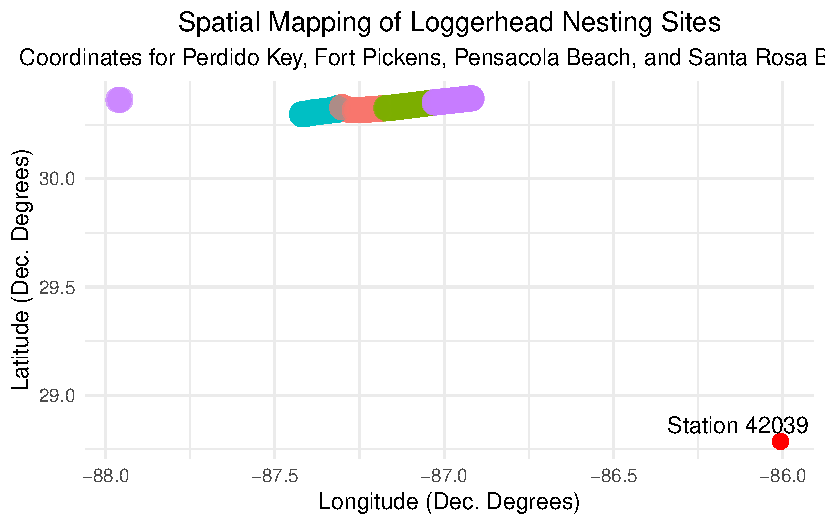
\includegraphics{RAWH_CAPSTONE_041926_files/figure-pdf/fig-spatial-1.pdf}

}

\caption{\label{fig-spatial}Spatial Mapping Of Loggerhead Nesting Sites
including Station 42039 Buoy Location}

\end{figure}%

\subsection{Mathematical and Statistical
Modelling}\label{mathematical-and-statistical-modelling}

Overall, Time Series Analysis is a layered methodology where each layer
can strengthen the fit and forecast of the overall model. The main steps
of the analysis include:

\begin{itemize}
\tightlist
\item
  Exploratory Data Analysis and Visualizations
\item
  Stationarity of Data
\item
  Decomposition Determination
\item
  Model Selection
\item
  Training and Validation
\item
  Metrics
\item
  Forecasting and Residual Analysis
\end{itemize}

\subsubsection{Exploratory Data Analysis and
Visualizations}\label{exploratory-data-analysis-and-visualizations}

The first series of analysis involves

\begin{itemize}
\tightlist
\item
  making sure the that the points are in time order and occurs at a
  consistent frequency
\item
  looking for patterns in the data and how the data changes over time
\item
  interpreting whether it contains a Trend or any Seasonality.
\end{itemize}

At this point, we also need to identify outliers and if they are
significant for the overall analysis or whether they should be trimmed.
It is also important to find any data that could be interpreted as ``not
applicable'' which would also skew the analysis with erroneous results,
for example, some data points may have ``n/a'', ``na'', or a
blank/missing value while others may put a number or letter sequence
that would not match with the rest of the data.

These errors in the data may not be discovered until plotting results.
Checking for linear relationships between two columns at a time may
reveal mistakes in the data set or erroneous values. I was able to
determine that several pairs of longitude and latitude points were
incorrectly recorded based on a simple spatial mapping plot of longitude
vs latitude. Since this is a collaborative effort with Dr.~Schmutz
(Professor of Earth and Environmental Science, UWF), he was notified so
that he could make the decision to omit the data or correct it; negative
signs were missing from the longitude data and he decided to correct
them. We found that all erroneous temperature readings recorded from the
buoy were the number `999' and so this had to be filtered out too
because the data would definitely be skewed.

\subsubsection{Stationarity of Data}\label{stationarity-of-data}

3 rules for strict stationarity\ldots{}

Constant Mean - an upward or downward trend denotes that the series is
not stationary.

Constant Variance - the volatility of the spread of the data should stay
consistent over the series. Increased deviations (fluctuations) from the
average as the series progresses shows non-stationarity.

Constant Autocorrelation - looking at time t and t-1 and the how they
differ; the difference of the internal structure/statistical properties
of the data should be constant and not significantly change over time.

The Augmented Dickey-Fuller (ADF) Test shows whether the data is
Stationary based on a resulting p-value. A Time Series Plot will confirm
the p-value of the ADF.

\subsubsection{Decomposition
Determination}\label{decomposition-determination}

Classical Decomposition Methods comprise of the Additive method and the
Multiplicative method.

For additive decomposition, the magnitude of the seasonal fluctuations
(or variation about the trend) are not expected to vary with the level
of the time series as the data grows, or shrinks, over time.
Essentially, we are assuming that there will be a constant absolute
magnitude about which there will be seasonal fluctuations.

An additive model's graphical representation will show that there will
be parallel peaks and troughs with a consistently even width between
them, respectively, even though the overall graph may be showing a
positive or negative correlation.

The components (S,T,R) are proven to be independent by performing an
additive decomposition and checking to see how R performs - if R
(remainder/noise) remains fairly consistent, then an additive
decomposition is needed; however, if R oscillates and increases in
magnitude (and continues to do so) then the multiplicative decomposition
has to be used.

\[ 
    y_t = S_t + T_t + R_t 
\] where S=Seasonal, T=Trend, R=Residuals/Noise at time \emph{t}

The multiplicative decomposition is used when the the magnitude of the
seasonal fluctuations are proportional to the level of the time series.
Essentially, there is a percentage change between the start and the end
of each season and, as aforementioned, the residuals are checked for
continually increasing oscillations.

\[ 
    y_t = S_t \times T_t \times R_t 
\] The STL method in R - Seasonal-Trend decomposition using Loess
(Locally Estimated Scatterplot Smoothing) to show the breakdown of S, T
and R.

The Trend Strength, \(F_t\), is the comparison of Remainder (\(R_t\))
versus the variance of the Data-without-Trend (\(T_t + R_t\)) and how
much data volatility there is in the long term. \[
F_m = max(0,1-[Var(R_t)/Var(m_t + R_t)])
\] The Seasonal Strength, \(F_s\), is the comparison of Remainder
(\(Y_t\)) versus the reduction in variance of the Seasonally-Adjusted
data (\(S_t + R_t\)) after the Trend has been removed. \[
F_s = max(0,1-[Var(R_t)/Var(s_t + R_t)])
\]

\subsubsection{Model Selection}\label{model-selection}

\begin{itemize}
\item
  SARIMAX (Seasonal Autoregressive Integrated Moving Average with an
  Exogenous Variable) is a comprehensive time series analysis that is a
  combination of seasonality, autoregression, differencing, moving
  average and is also a forecasting method that is well suited to a
  biological analysis. It is an extension of the ARIMA framework that
  incorporates the annual seasonality of biological data and the
  exogenous variable of water temperature. Also, like ARIMA, SARIMAX
  analysis data has to be proven stationary by testing its mean and
  variance to ensure that future predictions are based solidly on
  historical pattern recognition.

  \begin{itemize}
  \item
    The S (Seasonal) Component represents the \textbf{regular intervals}
    at which a relationship can be identified and is to be expected
    using biological data, i.e., finding the natural rythmn of the
    model.
  \item
    The AR (Autoregressive) Component, p, involves the model using the
    relationship of the variable with its own \textbf{previous values}
    (or lagged observations).
  \item
    The I (Integrated) Component, d, helps to \textbf{stabilize the
    mean} and remove trends from the time series analysis and makes it
    stationary by differencing (d).
  \item
    The MA (Moving Average) Component, q, represents the effect of
    \textbf{previous error} terms on the present value of the time
    series.
  \item
    The X (eXogenous) Component is an \textbf{external variable} that
    can help fill in the gaps of past behaviour of the data to soften
    fluctuations and strengthen future predictions. For this analysis,
    our exogenous variable is the Gulf of Mexico Surface Water
    Temperature.
  \item
    The SARIMAX model is mathematically represented using a Backshift
    (B) notation where \(By_t=y_{t-1}\):
  \end{itemize}
\end{itemize}

\[ 
    \Phi_P(B^s)\phi_p(B)\nabla^d\nabla_s^Dy_t=\beta x_t+\Theta_Q (B^s)\theta_q(B)\epsilon_t
\]

\textbf{-} \(y_t\): Dependent Variable, total nesting count

\textbf{-} \(x_t\): Exogenous Variable, surface water temperature

\textbf{-} \(\beta\): Coefficient, quantifies impact of water
temperature on nesting activity

\textbf{-} \(\nabla^d\) \textbf{and} \(\nabla_s^D\): Differencing
Operators

\textbf{-} \(\phi_p\) \textbf{and} \(\Phi_P\): AR(p) and SAR(P)
Components

\textbf{-} \(\theta_q\) \textbf{and} \(\Theta_Q\): MA(q) and SMA(Q)
Components

\textbf{-} \(\epsilon_t\): White Noise (error term)

\begin{itemize}
\item
  \textbf{Box-Jenkins time series method} has three steps that the time
  series analysis can be run through iteratively.

  \begin{itemize}
  \item
    \textbf{Step 1: Identification} determines the order of the Seasonal
    and non-seasonal AR, I and MA components that are appropriate for
    the time series and where the eXogenous variable is incorporated.
    Within this step, there is a Stationarity Check for stability using
    the mean and variance of the model and this includes determining the
    Seasonal Stationarity. If there are significant fluntuations in the
    Mean (from analyzing the peaks and troughs), Seasonal
    Differencing(D) is needed as well as Standard Differencing (d).
    Next, the Autocorrelation and Partial Autocorrelation Analysis (ACF
    and PACF) plots are generated to identify model lags or Seasonal
    Spikes (most probably a multiple of 12). The spikes will be used to
    identify the Seasonal Autoregressive (P) and Seasonal Moving Average
    (Q). The Seasonality Check of the data is to confirm that there is a
    repeating 12-month pattern, or biological cycle where s=12, thus,
    validating the ``S'' component in SARIMAX. The relationship between
    the Exogenous Variable (X) and the time series nedds to be
    identified appropriately such that it is statistically relavent and
    aligned (may have to impose a lag) to the overall model and can help
    explain the model's behaviour.
  \item
    \textbf{Step 2: Estimation} is where the a model is selected based
    on the identified seasonal and non-seasonal parameters \((p, d, q)\)
    x \((P,D,Q)_s\). The AR and MA lags are also selected based on the
    ACF and PACF found in the previous identification step. The
    non-seasonal AR (\(\phi\)) and MA coefficients (\(\theta\)) will be
    designated as well as the seasonal AR (\(\Phi\)) and MA (\(\Theta\))
    coefficients, if they exist. Lastly, for this step, the SARIMAX
    model's exogenous variable coefficient (\(\beta\)) can be estimated.
    All of these parameters will be applied and the model generates the
    fitted values to synthesize its unique historical behavior and
    predictive nature while amalgamating its historic patterns with the
    exogenous temperature data. The Akaike Information Criterion (AIC)
    will be used to make a parsimonious model to ensure accuracy using
    as few parameters as possible - too many parameters can diminish the
    model's optimization.
  \item
    \textbf{Step 3: Diagnostic Checking} involves investigating the
    residuals (the difference between the predicted SARIMAX values and
    observed data) to ensure no additional patterns are left in the
    error/residual terms; the residuals should resemble ``white noise''
    randomness. Next, the \textbf{Ljung-Box Test} is utilized to check
    to see if the residuals are as desired, i.e., random, followed by a
    mean and variance check; the desired outcome is that the residuals
    have a mean close to zero and a variance that is constant
    (homoskedasticity) confirming that the residuals do not grow or
    shrink over time. Also, the residuals are compared to the water
    temperature data to make sure that they do not correlate; if this is
    the case, its coefficient will have to be re-estimated. Finally, the
    term Iterative Refinement is used to describe the process for going
    back through the steps so far if the previous checks raised any
    issues.
  \end{itemize}
\item
  An \textbf{ACF Plot} will be generated to show the relationships
  within the data with respect to Seasonality and Non-stationary Trends.
  We will also be observing the prominence and regularity of the plot's
  spikes, if the mean is shifting over time by analyzing the correlation
  between data and lags, and whether Differencing is required to achieve
  stationarity.
\item
  A \textbf{PACF Plot} will be generated to determine the order of the
  standard AR (p) and the seasonal AR (P) via a ``cut-off'' point. A lag
  number will automatically be assigned for the SARIMAX model and the
  cut-off point should match this. This number is predicted to be 12
  since we are looking at biological data. Therefore, we will be paying
  attention to whether the cut-off at the beginning of the plot is 12
  which can lead to P being initially assigned a 1.
\item
  The automatic base model for ARIMA that is used during programming is
  of the format: \[ ARIMA(p,d,q)(P,D,Q)_{Lag}\] but is written within
  the report as: \[ SARIMAX(p,d,q)(P,D,Q)_{Lag}\]
\end{itemize}

\subsubsection{Training and Validation}\label{training-and-validation}

\begin{itemize}
\item
  Based on my research, SARIMAX, Fourier series, and Prophet all handle
  non-linear, highly seasonal data well. ``Neigbouring'' of the SARIMAX
  model will be used to make sure that a slight adjustment will not
  provide a better model.

  \begin{itemize}
  \item
    \textbf{SARIMAX} uses lags to its advantage and assumes high
    correlation with the previous 12-month instance to its current
    observation. It utilizes the Seasonal Moving Average or Seasonal
    Autoregressive terms by ``remembering'' historical biological
    patterns and distinguishing between a surge or an anomaly by taking
    full advantage of the environmental influence, i.e., the exogenous
    variable, of water temperature.
  \item
    \textbf{Fourier Series} is used in combination with ARIMA to create
    a Dynamic Harmonic Regression model. The Dynamic attribute uses ARMA
    to handle errors or ``memory'' in the data. The harmonic attribute
    explains how it is an approximation model that breaks down the data
    into the sum of sine and cosine functions to handle the seasonality
    component to aid in mapping a predictable cycle. The Regression
    attribute refers to the exogenous data and handles piece-wise shifts
    in nesting activities. The Fourier Series allows for a relaxed
    approach to defining biological seasonal cycles and is an excellent
    choice for biological data.
  \item
    \textbf{``Prophet''} was designed by the Data Science Team at Meta
    to handle fluctuations of business and biological data within time
    series analysis. Prophet decomposes the time series model using a
    Generalized Additive Model, or GAM, y(t) by Trend, g(t),
    Seasonality, s(t), Holidays/Events (e.g, Environmental Disasters),
    h(t), and an Error term, \(\epsilon_t\) - \$
    y(t)=g(t)+s(t)+h(t)+\epsilon\_t \$ - it then looks at the series and
    adjusts curves to show the relationship rather than analyzing the
    actual relationship between the data points. Prophet is known to
    handle missing data, more resilient to outliers, and extra exogenous
    variables can be added. It also incorporates the Fourier Series for
    the Seasonal aspect to generate a smoothed seasonal cycle.
  \item
    \textbf{``Neighboring''}, or Stepwise Evaluation of Neighboring
    Parameters, can be used as a comparison to validate the correctness
    of the chosen model, e.g., changing p=0 (no immediate memory) to p=1
    (1 month memory). Depending on what the SARIMAX model is, I will
    research what its ``neighbor'' should be and then test to make sure
    it is not better than the chosen model. There is also a balance to
    maintain between the simplicity and the accuracy of the model - one
    make the model as parsimonious as possible with the fewest number of
    parameters whilst maintaining accuracy.
  \end{itemize}
\item
  \textbf{Note:} Exponential Smoothing was considered but upon further
  research, it was not a good candidate because it can not handle the
  exogenous data well although it can generally handle outliers better
  than SARIMAX.
\end{itemize}

\subsubsection{Metrics}\label{metrics}

\begin{itemize}
\tightlist
\item
  \textbf{AIC (Akaike Information Criterion) score:} used to find the
  most parsimonious (efficient and simple) model from all of these
  methods; the lowest AIC score is usually the best but have to check
  the parameter count.
\item
  \textbf{``ma'' coefficients:} Moving Average coefficients are used to
  correct predictions from the previous point of the forecast, more
  likely to be a monthly forecast.
\item
  \textbf{``sma'' coefficient:} Seasonal Moving Average coefficients
  handles correcting predictions from the previous point of the
  forecast, more likely to be a yearly forecast.
\item
  \textbf{s.e. - Standard Error} measures the reliability of ALL of the
  coefficients generated. As a rule, if the coefficient being compared
  is roughly double that of the standard error, the coefficient is
  deemed statistically significant corresponding to a \(p-value\) of
  0.05.
\item
  \textbf{sigma2 - \(\sigma^2\)} is the variance of the residuals, or
  remaining noise, in the model that can not be explained. A lower
  \(\sigma^2\) suggests a better, tighter fit.
\item
  \textbf{RMSE - Root Mean Squared Error} is a measure of trust in the
  model's predictions. It averages the distance between the model's
  predictions against the original observed data. The RMSE will be in
  the same units as the data which, in our case, is number of nests.
\end{itemize}

\subsubsection{Forecasting and Residual
Analysis}\label{forecasting-and-residual-analysis}

\begin{itemize}
\tightlist
\item
  \textbf{Train and Test} - we will use the first 21 years (1988-1999)
  of the data to develop the training model and the last year year of
  data will be used as the test set for each model's forecasting
  capabilities. This is called the ``Out-of-Sample Validation''.
\item
  \textbf{Forecasting} - this is a probabilistic estimate of what the
  future of the model will look like based on the patterns learned
  during training. Point Forecasts that offer its best estimate as to
  where future data points will reside in future months. Prediction
  Intervals consist of 80\% and 95\% uncertainty ranges that show the
  variability in nesting counts based on past learning of fluctuations
  or ``environmental shocks''.
\item
  \textbf{Residual Analysis} - after forecasting, the residuals
  behaviour will be compared to ``White Noise'' and will be verified
  using a Ljung-Box Test and a Residual Histogram to check for model
  bias and that the residuals are at a minimum.
\end{itemize}

\subsection{Software and Tools}\label{software-and-tools}

\begin{itemize}
\tightlist
\item
  R Programming Environment - widely used for time series analysis.
\item
  fpp3 ``Forecasting:Principles and Practice'' meta-package.
\item
  tsibble - creation and management of data frames.
\item
  feasts - ``Feature Extraction and Statistics for Time Series'', used
  for calculating the Ljung-Box p-value.
\item
  fable - primary modeling entity for defining, estimating, and
  forecasting SARIMAX and Fourier ARIMA models.
\item
  fable.prophet - to incorporate the Generalized Additive Model (GAM)
\item
  STL method - Seasonal-Trend decomposition using Loess (Locally
  Estimated Scatterplot Smoothing).
\end{itemize}

\subsection{Ethical Considerations}\label{ethical-considerations}

Data integrity and Transparency

Conservation Policies

Sensitive Information/Species Protection

\section{Results}\label{results}

The analysis addresses the extent at which the nesting trends are
changing with respect to:

\begin{itemize}
\tightlist
\item
  time
\item
  water temperature (possible sex imbalance inference)
\end{itemize}

\subsection{Core Findings}\label{core-findings}

\subsubsection{Exploratory Data Analysis and
Visualizations}\label{exploratory-data-analysis-and-visualizations-1}

\begin{itemize}
\item
  Individual yearly plots were generated to show the yearly nesting
  patterns compared to the 22-year average (see
  Figure~\ref{fig-ind-plots}).
\item
  2017 had the highest number of nesting sites (see
  Figure~\ref{fig-total-nesting-year})
\item
  Perdido Key had the most nesting sites (see
  Figure~\ref{fig-beach-table})
\item
  July was the aggregated top month for nesting sites (see
  Figure~\ref{fig-top-month})
\item
  The seasonality of the data can be observed (see@tbl-CCseason-table)
\item
  ANOVA results using Tukey Honest Significant Difference (HSD) or
  Comparison of the Means (95\% confidence level), (see
  Table~\ref{tbl-buoy-tukey-table})
\item
  Relative Relationship between Nesting Activity and Average monthly
  temperatures show a high correlation (see
  Figure~\ref{fig-relative-nest-temp}).
\item
  The plot, shown below, shows the relationship between the water
  temperature and nesting activity. The water temperature was scaled and
  the nesting activity was normalized so that they could use the same
  Relative Intensity scale.
\end{itemize}

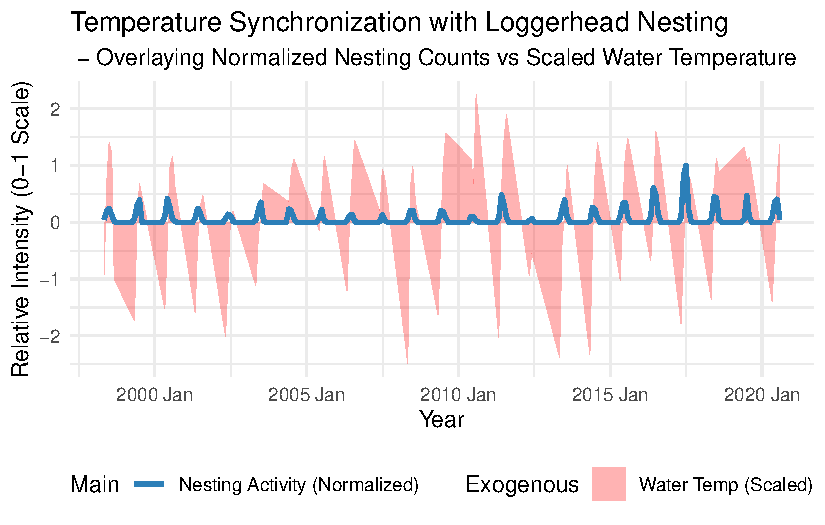
\includegraphics{RAWH_CAPSTONE_041926_files/figure-pdf/unnamed-chunk-9-1.pdf}

\subsubsection{Stationarity of Data}\label{stationarity-of-data-1}

\begin{itemize}
\item
  Null Hypothesis, \(H_0\): The data is non-stationary and contains a
  unit root
\item
  Alt. Hypothesis, \(H_1\): The data is stationary and does not contain
  a unit root
\item
  Fail to Reject the Null Hypothesis iff p \textgreater{} 0.05
\item
  The Augmented Dickey-Fuller (ADF) Test Results

  \begin{itemize}
  \tightlist
  \item
    for \textbf{Nesting Activity, p = 0.0868}, and
  \item
    for \textbf{Average Gulf Surface Temperature, p = 0.1000}.
  \end{itemize}
\item
  Conclusion: We Fail to Reject the Null Hypothesis; \textbf{both sets
  of data are non-stationary} and the data must be stabilized.
\end{itemize}

\begin{itemize}
\tightlist
\item
  A Time Series Plot was configured and it showed that the \textbf{Mean
  and Variance were NOT constant} due to the peaks and valleys, i.e.,
  confirming evidence that the data is Non-Stationary.
\end{itemize}

\subsubsection{Decomposition
Determination}\label{decomposition-determination-1}

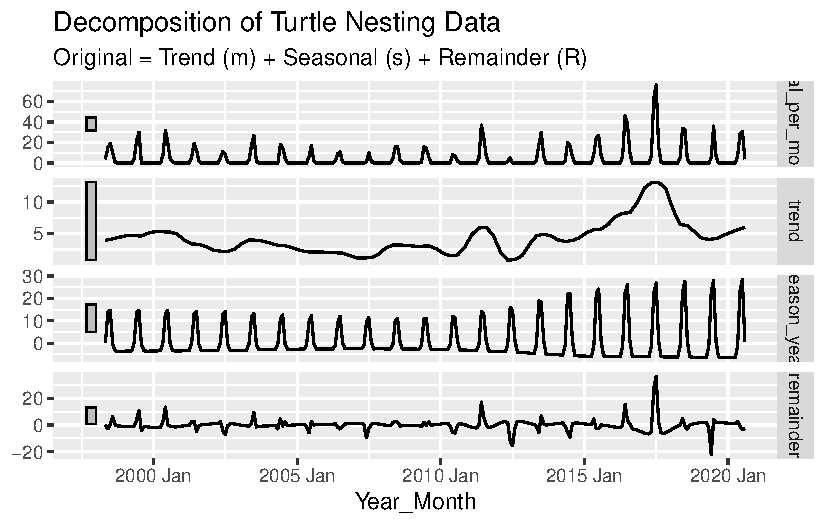
\includegraphics{RAWH_CAPSTONE_041926_files/figure-pdf/unnamed-chunk-11-1.pdf}

\begin{itemize}
\tightlist
\item
  This is an example of Multiplicative Decomposition because the
  Residuals, or Remainder, (Y) are not constant over time and are larger
  as the number of nests increase showing that the seasonal variance is
  proportional to the trend. The Seasonal component shows a very regular
  pattern. The Trend is showing a very slight upward relationship and
  could infer that conditions are becoming more favorable for nesting
  turtles. The trend has successfully captured the the full growth
  pattern of the data (including the notably large nesting month in
  2017) and has ignored the month-to-month bumps. However, because the
  trend has a large bump, and not a completely horizontal line, shows
  the need for Differencing in the SARIMAX Model.\\
\item
  The Nesting Trend Strength is 0.3163 (0.6 minimum) and considered weak
  in the SARIMAX model. Unfortunately, this does not bode well for
  nesting turtles since this shows that there is not a consistent upward
  trend, although spikes over the years are observed and more are
  possible in the future.
\item
  The Strong Nesting Seasonal Strength (0.7951) shows that there is a
  highly predictable season and can be seen directly in
  Table~\ref{tbl-CCseason-table}.
\end{itemize}

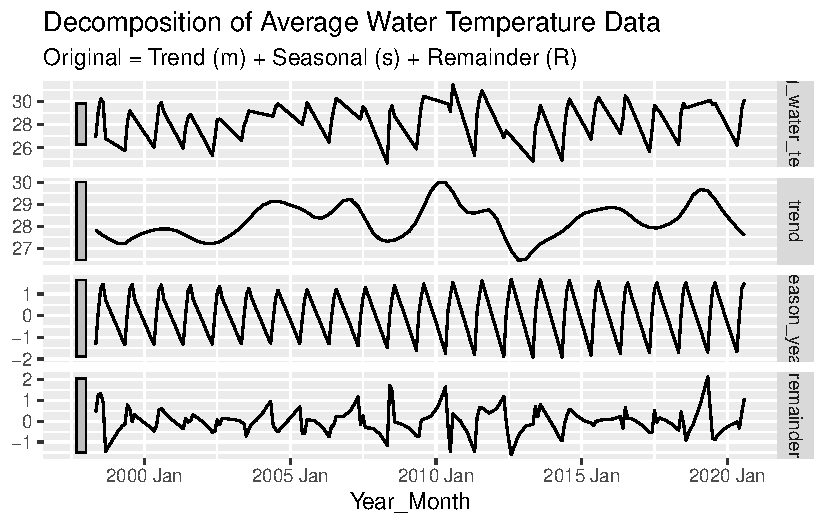
\includegraphics{RAWH_CAPSTONE_041926_files/figure-pdf/unnamed-chunk-13-1.pdf}

\begin{itemize}
\tightlist
\item
  This is also an example of Multiplicative Decomposition because the
  Residuals, or Remainder, (Y) are not constant over time. The Seasonal
  component shows a very regular pattern. The Trend is showing an upward
  relationship and could infer that water temperatures are getting
  warmer over the the two decades of data. The month-to-month trend
  bumps have been smoothed out but the swings are very noticeable and
  shows the need for Differencing in the SARIMAX Model.
\item
  The Average Water Temperature Trend Strength is 0.7618 which is
  considered strong. Unfortunately, this does not bode well for nesting
  turtles since this shows that the sea surface temperatures are on an
  upward trend which may interfere with the sex imbalance within turtle
  populations.

  \begin{itemize}
  \tightlist
  \item
    The Strong Nesting Seasonal Strength (0.7571) shows that there is a
    highly predictable season and can also be seen directly in
    Table~\ref{tbl-CCseason-table}.
  \end{itemize}
\end{itemize}

\begin{itemize}
\tightlist
\item
  There is Differencing Loss in the model. The use of the Seasonal
  Differencing (D=1) makes the model disregard the first 12 months of
  data since it has no previous time to compare with.
\end{itemize}

\subsubsection{Model Selection}\label{model-selection-1}

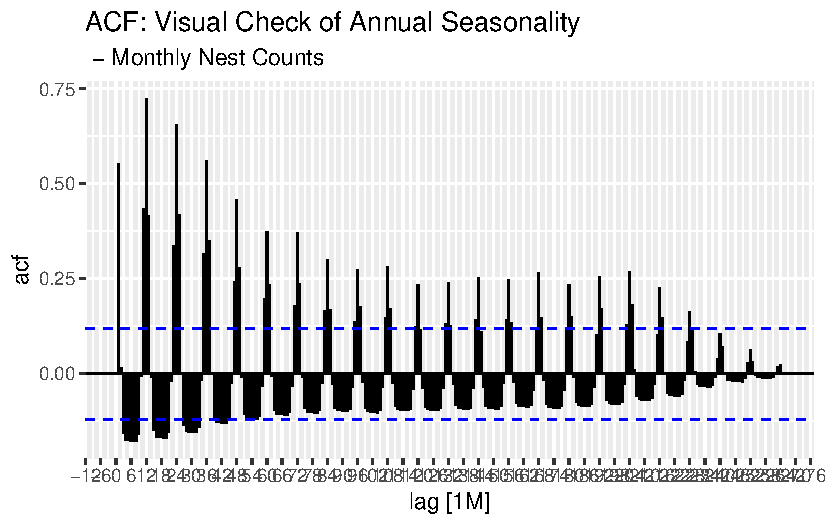
\includegraphics{RAWH_CAPSTONE_041926_files/figure-pdf/unnamed-chunk-15-1.pdf}

\begin{itemize}
\tightlist
\item
  The Nesting ACF Plot shows that there is Seasonality in the data
  showing yearly peaks. There is a definite trend since the bars stay
  high and decrease slowly over all lags. This also shows that the mean
  is shifting over time and Differencing is required for SARIMAX
  modelling.
\end{itemize}

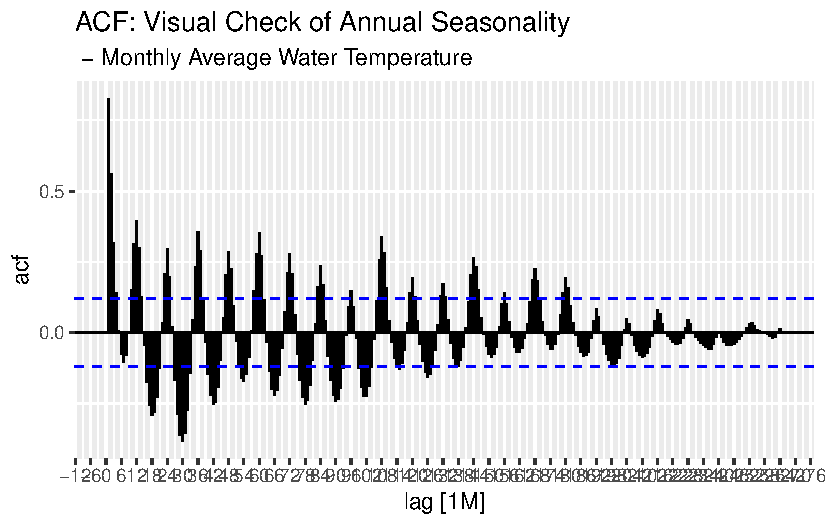
\includegraphics{RAWH_CAPSTONE_041926_files/figure-pdf/unnamed-chunk-16-1.pdf}

\begin{itemize}
\tightlist
\item
  The Water Temperature ACF Plot shows that there is Seasonality in the
  data showing varied yearly peaks. There is a trend since the bars
  generally stay high and decrease slowly over all lags with minor
  fluctuations. This corresponds to the mean shifting over time and
  supports that Differencing is required for the SARIMAX model.
\end{itemize}

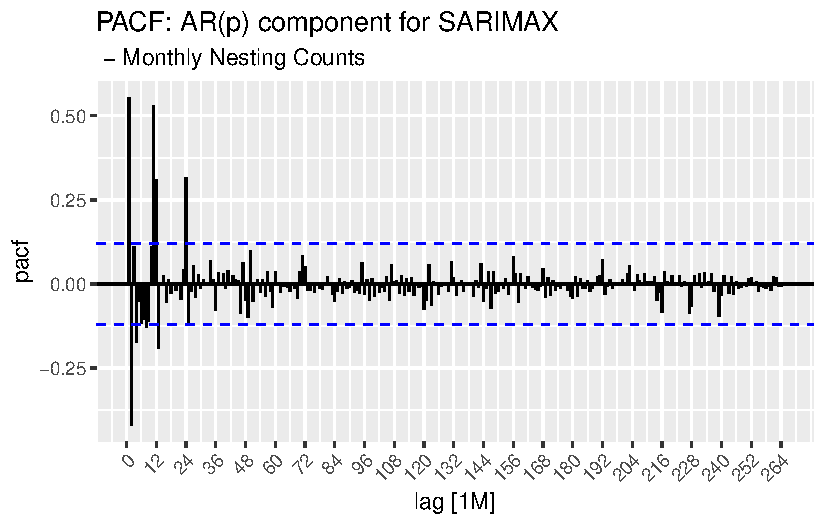
\includegraphics{RAWH_CAPSTONE_041926_files/figure-pdf/unnamed-chunk-17-1.pdf}

\begin{itemize}
\tightlist
\item
  The PACF determines the order of AR via a ``cutoff'' point. The last
  significant cutoff point in the plot is at the 48 month mark after
  which the spikes are in, or very close to, the ``insignificant zone''
  and is akin to ``white noise''. This shows there is some direct
  correlation with the data's own past values at the same time the
  previous year; therefore, p = 0.
\end{itemize}

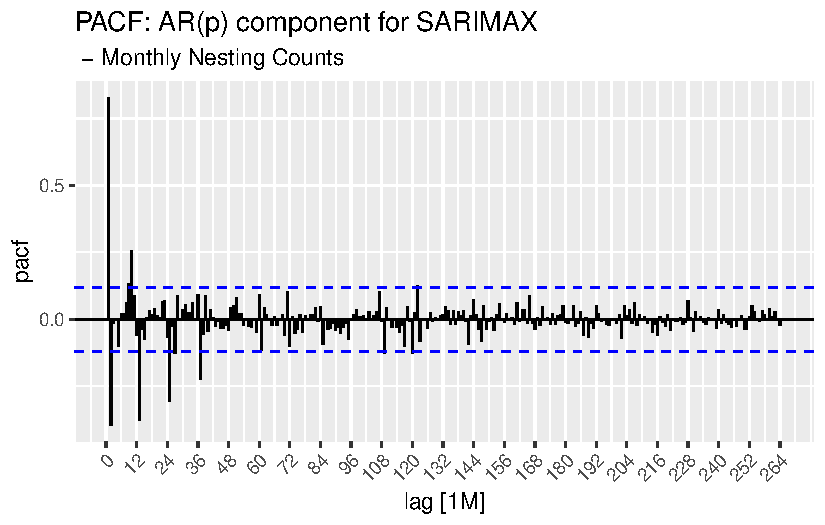
\includegraphics{RAWH_CAPSTONE_041926_files/figure-pdf/unnamed-chunk-18-1.pdf}

\begin{itemize}
\tightlist
\item
  The last significant cutoff point in the Temperature ACF plot is at
  the 36 month mark after which the spikes are in the ``insignificant
  zone'' and is akin to ``white noise''. This shows there is some direct
  correlation with the data's own past values at the same time the
  previous year; therefore, p = 0 still holds for the overall model
  behaviour.
\end{itemize}

\begin{table}
\caption*{
{\fontsize{20}{25}\selectfont  SARIMA Automatic Modelling Coefficients\fontsize{12}{15}\selectfont } \\ 
{\fontsize{14}{17}\selectfont  - ARIMA(0,0,2)(0,0,1)[12] for Nesting Activity\fontsize{12}{15}\selectfont }
} 
\fontsize{12.0pt}{14.0pt}\selectfont
\begin{tabular*}{\linewidth}{@{\extracolsep{\fill}}lrrr}
\toprule
Parameter & Coefficient & Std. Error & z-value \\ 
\midrule\addlinespace[2.5pt]
ma1 & 0.6001480 & 0.06212687 & 9.660039 \\ 
ma2 & 0.1378960 & 0.06141272 & 2.245397 \\ 
sma1 & -0.6977397 & 0.05465797 & -12.765562 \\ 
\bottomrule
\end{tabular*}
\end{table}

\begin{itemize}
\tightlist
\item
  The automatically-fitted model gives us ARIMA(0,0,2)(0,0,1){[}12{]}
  and the backshift equation is as follows:
\end{itemize}

\[
    y_t=(1+\theta_1 B+ \theta_2 B^2)(1+\Theta_1 B^{12})\epsilon_t
\] - However, the ADF test shows that the model is non-stationary and is
in need of Differencing. We must keep the model as parsimonious as
possible but the model is invalid in its current form. Adding
Differencing, D = 1, will satisfy the requirement to stabilize the data
and, also, flatten out the mean over time. This model will be tested as
a ``neighbor'' model during training and validation stage to verify its
fit. Adding the Differencing adds a term to the left side of the model
equation and mathematically interprets the annual changes in turtle
nesting as shown below: \[
    (1-B^{12})y_t=(1+\theta_1 B+ \theta_2 B^2)(1+\Theta_1 B^{12})\epsilon_t
                 =(1+0.6B+ 0.14B^2)(1-0.7B^{12})\epsilon_t
\]

\textbf{-} ma1 = 0.60 (s.e. = 0.063, significant since ma1
\textgreater{} 2*se)

\textbf{-} ma2 = 0.14 (s.e. = 0.062, significant since ma2
\textgreater{} 2*se)

\textbf{-} sma1 = -0.70 (s.e. = 0.058, significant since
\textbar sma1\textbar{} \textgreater{} 2*se )

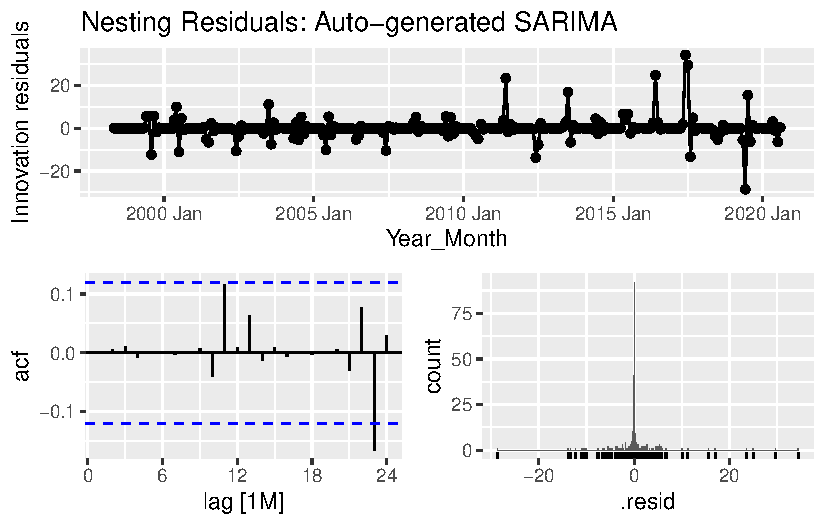
\includegraphics{RAWH_CAPSTONE_041926_files/figure-pdf/unnamed-chunk-20-1.pdf}

\begin{itemize}
\item
  The ARMA, or Autoregression (AR) and Moving Average (MA), base
  accounts for zero AR terms and a two month MA. The AR is zero because
  of the strong seasonality of the model (PQ has more influence). Also,
  the exogenous surface water temperature shows that it holds the
  momentum of the monthly nesting activity and provides an innate
  seasonality to the model.
\item
  The S in SARIMA includes Seasonality to the ARIMA model; P, D, and Q
  define the Seasonality of the model as well as the Differencing needed
  to stabilize the mean.
\item
  The X in SARIMAX adds the exogenous (external) variable of Surface
  Water Temperature and also adds an environmental influence.
\item
  The final SARIMAX equation with respect to Nesting Activity, and
  including Differencing, is as follows:
\end{itemize}

\[ SARIMAX(p,d,q)(P,D,Q)_{AnnualLag} = SARIMAX(0,0,2)(0,1,1)_{12} \]

\begin{itemize}
\item
  Difference: \textbf{d = 0}, although the mean was not a flat
  horizontal line, it was stable across of the series. Adding d = 1
  makes the model less parsimonious, therefore less efficient, and
  avoids over-differencing which almost always leads to overfitting.
\item
  Seasonal Difference: \textbf{D = 1}, due to strong Seasonal Strength
  of both the nesting activity and the water temperature, the model is
  strong enough to drive its own seasonality; it could also be that the
  dip in 2019 nesting activity could have been the slight disruption
  that set D = 0.
\item
  Autoaggressive: \textbf{p = 0}, the number of nests found in one month
  does not have a ripple effect from the previous month possibly because
  turtles nest up to every two weeks (on average) during a season but
  only make an average of 4 nests over a maximum season of 5 months.
\item
  Seasonal Autoaggressive: \textbf{P = 0}, the number of nests found in
  one season does not have a ripple effect from the previous season
  possibly because turtles nest every two or more years (on average).
\item
  Moving Average: \textbf{q = 2}, the model has memory from the previous
  2 months to adjust for the current month.
\item
  Seasonal Moving Average: \textbf{Q = 1}, the model is able to adjust
  for inconsistencies in nest counts from last year to the current
  year's prediction. Inconsistencies can arise from weather deviations
  like cold snaps or hurricanes and other environmental disasters like
  the Gulf oil spill of Summer, 2010.
\item
  Checking Residuals: shows the graphical representation of the
  residuals. The following analysis proves that the Auto-generated ARIMA
  can be considered an accurate representation of the model.

  \begin{itemize}
  \tightlist
  \item
    The Innovation Residuals show that the minor ``shock'' fluctuations
    mostly remain around a zero-mean like ideal ``White Noise''. The
    unexpected negative influence (significant innovation or ``shock'')
    at the end of the system shows that the model was not expecting the
    lower nesting numbers. The equation below explains how the
    ``shocks'' that occur in the system are represented to account for
    unpredictable fluctuations after seasonal and trend instances have
    been accounted for.
  \end{itemize}
\end{itemize}

\[ 
    \epsilon_t = y_t - E[y_t|PastInformation] 
\]

\begin{itemize}
\item
  Using the Ljung-Box Test (ACF Analysis), the lack of lag spikes
  outside of the boundaries of the ACF of Residuals shows that the model
  contains most of the information from the data and what is left
  consists mostly of random noise. The ACF plot confirms that the
  residuals are made up of white noise and are considered uncorrelated.
  The model can be viewed as a success given that the spikes at 12 and
  24 are within the ``insignificant'' zone. There is one spike at 23
  months that is most likely to be an example of mathematical
  ``shadowing'' or an interaction/cross-product. The cross-product is
  formed from multiplying terms from the model equation that represents
  the non-seasonal MA (2) and the seasonal MA (1), in our case,
  \((1+\theta_1 B+\theta_2 B^2) \times (1+\Theta_1 B^{12})\). The
  resulting interaction terms, \(B^{S\pm 1}\) and \(B^{S\pm 2}\),
  mathematically explain the second-order shadowing effect observed at
  Lag 23 (2S-1, for S=12). This is a known property of multiplicative
  models as established by Box (\citeproc{ref-BoxJenkins1970}{1970}).
  The spike at Lag 23 is not a representation of an omitted seasonal
  cycle but a mathematical resonance of the 12 and 11 month dependencies
  and so can be ignored now that it has been accounted for.
\item
  The Residual Histogram (count vs residuals) shows that the residuals
  are centered about zero and follows a fairly normal (bell-shaped)
  distribution suggesting that the model is unbiased.
\item
  In conclusion, the three plots encapsulate the idea that all available
  patterns have been captured. The residuals have shown to be
  uncorrelated and normally distributed allowing the confidence levels
  to expand over time at a realistic rate during extended forecasting
  (see (\citeproc{ref-sarima-fit-auto}{\textbf{sarima-fit-auto?}})).
\end{itemize}

\subsubsection{Training and Validation}\label{training-and-validation-1}

\begin{itemize}
\item
  The base\_sarimax and pdq\_sarimax (has p-d-q-P-D-Q values hard-coded
  into its model) achieved the best overall performance with an Akaike
  Information Criterion (AIC) of 1544.76 for all data from 1988 to 2018.
  The data for 2020 is set aside to be used to evaluate the model's
  performance on new unseen data. The negatively-influenced nesting
  season of 2020 will test the robustness of the model's ability to
  forecast effectively and accurately.
\item
  I ran both base\_sarimax and pdq\_sarimax to check that they had the
  same AIC result, then remove pdq\_sarimax to simplify the table.
\item
  Per the R-Studio-generated warning, ``automatic selection does not
  select models with characteristic roots that may be numerically
  unstable''(\citeproc{ref-fpp3}{Hyndman and Athanasopoulos 2026}). The
  base\_arima with Box-Cox (lambda = 0, log transform), Fourier 1, GAMs,
  and Prophet could not predict a model because a small change in data
  could make the model unstable. R-Studio ignores the unstable models
  and will choose something more reliable that will work in the
  long-term.
\end{itemize}

\begin{table}
\caption*{
{\fontsize{20}{25}\selectfont  Models AICc Scores (Ranked Lowest to Highest)\fontsize{12}{15}\selectfont } \\ 
{\fontsize{14}{17}\selectfont  - Partial Dataset, 1998-2019\fontsize{12}{15}\selectfont }
} 
\fontsize{12.0pt}{14.0pt}\selectfont
\begin{tabular*}{\linewidth}{@{\extracolsep{\fill}}lccccc}
\toprule
Model & AIC & AICc & BIC & Log Likelihood & Sigma Squ. \\ 
\midrule\addlinespace[2.5pt]
n\_sarimax\_002\_011 & 1437.11 & 1437.28 & 1450.96 & -714.55 & 24.62 \\ 
temp\_sarimax\_002\_011 & 1438.26 & 1438.52 & 1455.58 & -714.13 & 24.63 \\ 
auto\_sarimax & 1438.75 & 1439.25 & 1463.00 & -712.38 & 24.49 \\ 
temp\_sarimax & 1440.17 & 1440.80 & 1467.88 & -712.08 & 24.53 \\ 
fourier\_sarimax\_5 & 1500.54 & 1502.90 & 1556.76 & -734.27 & 23.02 \\ 
fourier\_sarimax\_6 & 1502.54 & 1505.20 & 1562.27 & -734.27 & 23.12 \\ 
fourier\_sarimax\_4 & 1504.21 & 1506.01 & 1553.40 & -738.11 & 23.51 \\ 
fourier\_sarimax\_3 & 1518.99 & 1520.32 & 1561.15 & -747.50 & 25.05 \\ 
fourier\_sarimax\_2 & 1539.44 & 1540.37 & 1574.57 & -759.72 & 27.28 \\ 
temp\_sarimax\_002\_001 & 1625.56 & 1625.91 & 1646.64 & -806.78 & 39.55 \\ 
sarimax\_002\_001 & 1631.76 & 1632.01 & 1649.33 & -810.88 & 40.69 \\ 
gam\_fourier\_4 & 1636.81 & 1637.73 & 1671.94 & -808.40 & 41.20 \\ 
ets\_model & 2262.00 & 2264.07 & 2314.71 & -1116.00 & 34.63 \\ 
base\_snaive & NA & NA & NA & NA & 49.45 \\ 
\bottomrule
\end{tabular*}
\end{table}

\subsubsection{Forecasting}\label{forecasting}

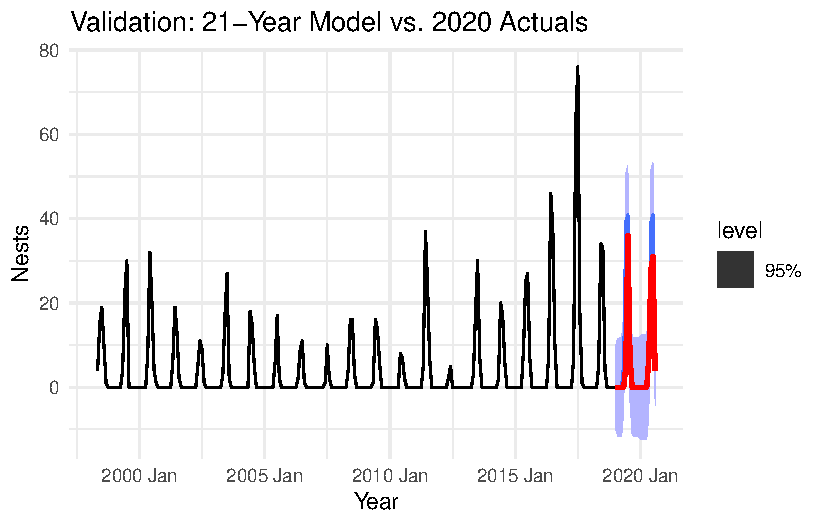
\includegraphics{RAWH_CAPSTONE_041926_files/figure-pdf/unnamed-chunk-23-1.pdf}

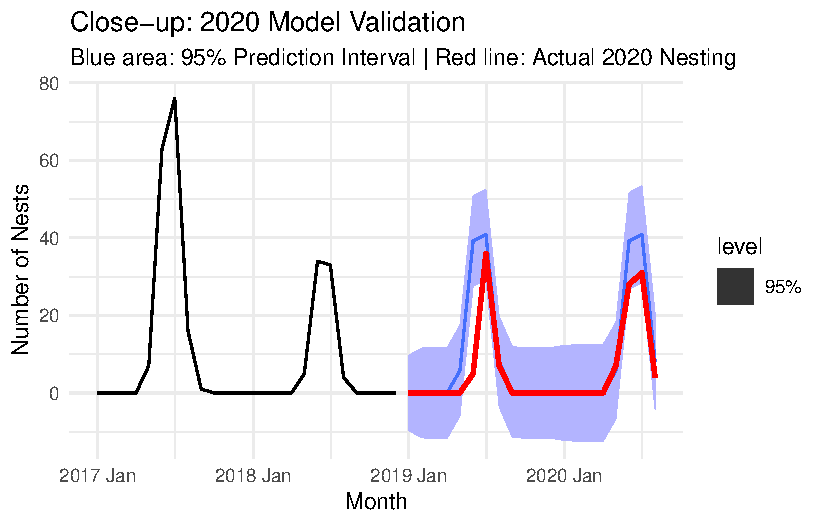
\includegraphics{RAWH_CAPSTONE_041926_files/figure-pdf/unnamed-chunk-24-1.pdf}

\subsubsection{Metrics}\label{metrics-1}

\begin{table}
\caption*{
{\fontsize{20}{25}\selectfont  Ljung-Box Residual Test Results\fontsize{12}{15}\selectfont } \\ 
{\fontsize{14}{17}\selectfont  - n\_sarimax\_002\_011\fontsize{12}{15}\selectfont }
} 
\fontsize{12.0pt}{14.0pt}\selectfont
\begin{tabular*}{\linewidth}{@{\extracolsep{\fill}}lrr}
\toprule
Model & Q-Statistic & p-value \\ 
\midrule\addlinespace[2.5pt]
n\_sarimax\_002\_011 & 10.63584 & 0.9694178 \\ 
\bottomrule
\end{tabular*}
\end{table}

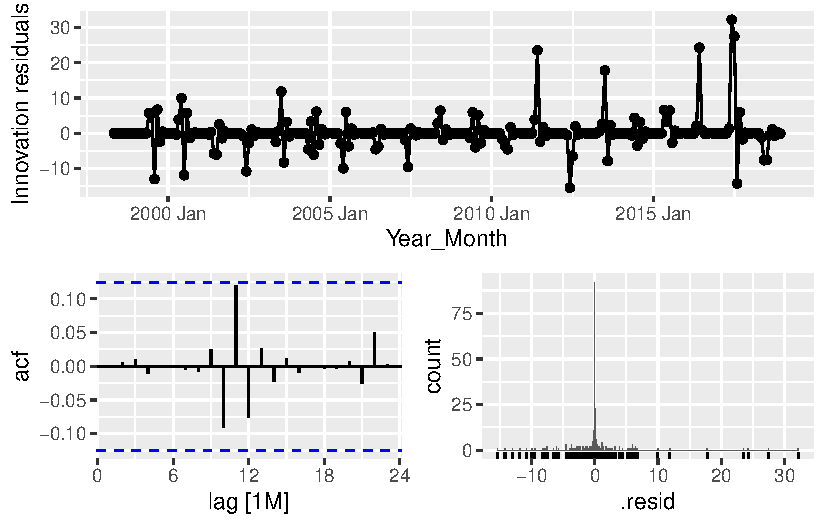
\includegraphics{RAWH_CAPSTONE_041926_files/figure-pdf/unnamed-chunk-26-1.pdf}

\begin{itemize}
\tightlist
\item
  Only 3 parameters (degrees of freedom) used: q=2 (ma1, ma2) and D=1,
  Q=1, (sma1).
\item
  With greater than 0 parameters used, the independence from the
  residuals is confirmed and the model is not over-fitted.
\item
  The p\_value is greater than 0.05, we fail to reject the Null
  Hypothesis which mathematically proves that the residuals are White
  Noise.
\item
  After applying the Ljung-Box test have officially passed the
  ``base\_sarimax''. \[
    dof = TotalLags-(p+q+P+Q)=24-3=21
  \]
\end{itemize}

\begin{table}
\caption*{
{\fontsize{20}{25}\selectfont  Root Mean Squared Error \& Mean Average Error\fontsize{12}{15}\selectfont } \\ 
{\fontsize{14}{17}\selectfont  - n\_sarimax\_002\_011\fontsize{12}{15}\selectfont }
} 
\fontsize{12.0pt}{14.0pt}\selectfont
\begin{tabular*}{\linewidth}{@{\extracolsep{\fill}}lrr}
\toprule
Model & RMSE & MAE \\ 
\midrule\addlinespace[2.5pt]
n\_sarimax\_002\_011 & 8.578671 & 3.636515 \\ 
\bottomrule
\end{tabular*}
\end{table}

\begin{itemize}
\tightlist
\item
  The average number of nests that the model prediction is ``off'' is 8
  which is a good result.
\end{itemize}

\subsection{Model Performance and
Comparisons}\label{model-performance-and-comparisons}

\[
  y_t=\beta(Temperature_t) +\eta_t
\] where \(\eta_t\) is an ARIMA process

\subsection{Uncertainty and
Variability}\label{uncertainty-and-variability}

TBD

\section{Discussion}\label{discussion}

\subsection{Interpretation}\label{interpretation}

Notice the sharp downward spike in the remainder at the very end (late
2019/2020). This suggests that the actual nesting was much lower than
the model expected for that time of year. This is a great point for your
Discussion section---you can investigate if there was a late-season
storm or a temperature drop that caused this deviation.

\subsection{Limitations and
Challenges}\label{limitations-and-challenges}

No new data after 2020 available.

\subsection{Implications}\label{implications}

The unbiased nature of the model is very important when used with
respect to conservation efforts. Since the residuals are centered about
zero, the model can estimate the population fairly accurately without
over- or under-estimating. This provides a realistic baseline for the
nesting activity of the Loggerhead Turtles resulting in informed
protection efforts and more precise resource allocation along the Gulf
Coast.

\section{Conclusion}\label{conclusion}

\subsection{Conclusion}\label{conclusion-1}

TBD

\subsection{Future Work}\label{future-work}

\begin{table}
\caption*{
{\fontsize{20}{25}\selectfont  Top 5 Models AICc Scores (Ranked)\fontsize{12}{15}\selectfont } \\ 
{\fontsize{14}{17}\selectfont  - Complete Dataset, 1998-2020\fontsize{12}{15}\selectfont }
} 
\fontsize{12.0pt}{14.0pt}\selectfont
\begin{tabular*}{\linewidth}{@{\extracolsep{\fill}}lccccc}
\toprule
Model & AIC & AICc & BIC & Log Likelihood & Sigma Squ. \\ 
\midrule\addlinespace[2.5pt]
auto\_full & 1588.06 & 1588.22 & 1602.24 & -790.03 & 27.48 \\ 
neighbor\_full\_1 & 1588.06 & 1588.22 & 1602.24 & -790.03 & 27.48 \\ 
temp\_full & 1589.79 & 1590.03 & 1607.52 & -789.90 & 27.55 \\ 
temp\_full\_1 & 1589.79 & 1590.03 & 1607.52 & -789.90 & 27.55 \\ 
f100\_sarimax\_5 & 1642.51 & 1644.68 & 1699.97 & -805.26 & 25.09 \\ 
\bottomrule
\end{tabular*}
\end{table}

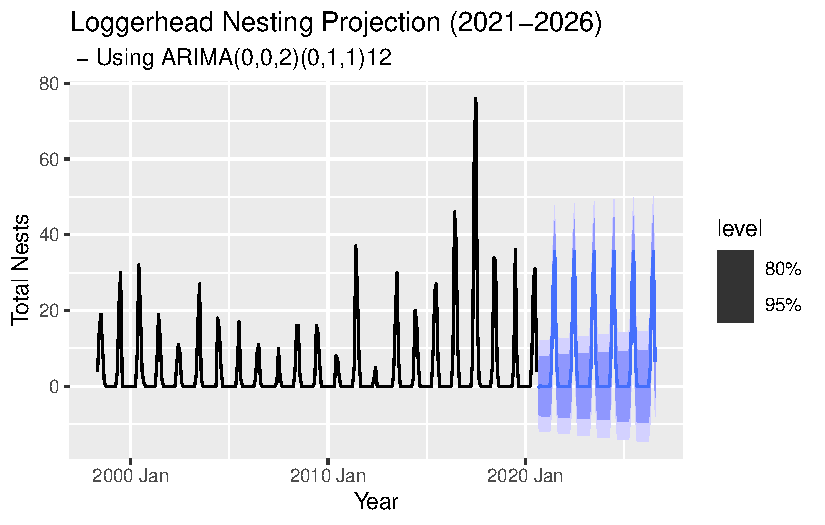
\includegraphics{RAWH_CAPSTONE_041926_files/figure-pdf/unnamed-chunk-29-1.pdf}

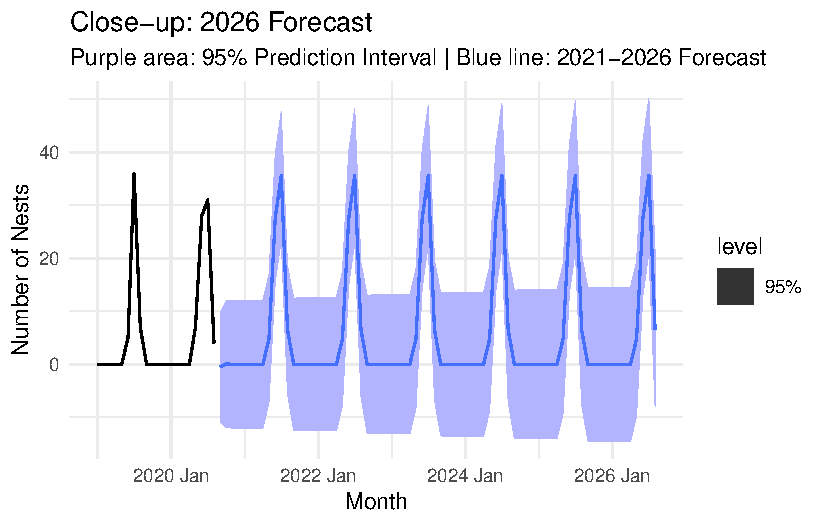
\includegraphics{RAWH_CAPSTONE_041926_files/figure-pdf/unnamed-chunk-30-1.pdf}

\subsection{Additional Visualization and
Tables}\label{additional-visualization-and-tables}

\begin{figure}

\centering{

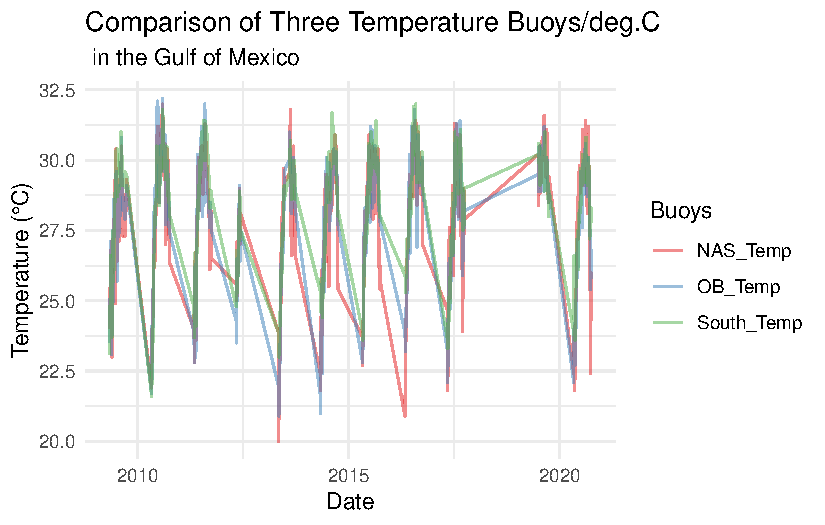
\includegraphics{RAWH_CAPSTONE_041926_files/figure-pdf/fig-buoy-comp-1.pdf}

}

\caption{\label{fig-buoy-comp}Comparison of Three Temperature
Buoys/deg.C}

\end{figure}%

\begin{table}

\caption{\label{tbl-buoy-tukey-table}Tukey HSD Comparison of Mean Water
Temperatures}

\centering{

\centering
\begin{tabular}[t]{l|r|r|r|r}
\hline
Comparison & Difference (degC) & Lower Bound & Upper Bound & p-adj\\
\hline
OB\_Temp-NAS\_Temp & -0.0131 & -0.2010 & 0.1748 & 0.9854\\
\hline
South\_Temp-NAS\_Temp & 0.2141 & 0.0262 & 0.4020 & 0.0207\\
\hline
South\_Temp-OB\_Temp & 0.2272 & 0.0393 & 0.4151 & 0.0128\\
\hline
\end{tabular}
\centering
\begin{tabular}[t]{l|l|l|l|l|l|l|l}
\hline
var & type & column\_label & column\_units & column\_pattern & column\_align & column\_width & hidden\_px\\
\hline
Comparison & default & Contrast & NA & NA & left & NULL & NULL\\
\hline
Difference (degC) & default & Difference (degC) & NA & NA & right & NULL & NULL\\
\hline
Lower Bound & default & Lower Bound & NA & NA & right & NULL & NULL\\
\hline
Upper Bound & default & High Bound & NA & NA & right & NULL & NULL\\
\hline
p-adj & default & Adj. p\_value & NA & NA & right & NULL & NULL\\
\hline
\end{tabular}
\centering
\begin{tabular}[t]{r|l|l|l|l|l}
\hline
rownum\_i & row\_id & group\_id & group\_label & indent & built\_group\_label\\
\hline
1 & NA & NA & NULL & NA & NA\\
\hline
2 & NA & NA & NULL & NA & NA\\
\hline
3 & NA & NA & NULL & NA & NA\\
\hline
\end{tabular}
\centering
\begin{tabular}[t]{l}
\hline
x\\


\hline
\end{tabular}\begin{table}
\caption{NA}

\centering
\begin{tabular}[t]{l}
\hline
x\\
\hline
Tukey HSD Comparison of Mean Gulf Water Temperature\\
\hline
\end{tabular}
\centering
\begin{tabular}[t]{l}
\hline
x\\
\hline
95\% Confidence Level\\
\hline
\end{tabular}
\centering
\begin{tabular}[t]{}
\hline

\hline
\end{tabular}
\end{table}
\centering
\begin{tabular}[t]{l|l|l|l|l|r|l|l}
\hline
vars & spanner\_label & spanner\_units & spanner\_pattern & spanner\_id & spanner\_level & gather & built\\


\hline
\end{tabular}\begin{table}
\caption{NA}

\centering
\begin{tabular}[t]{}
\hline

\hline
\end{tabular}
\end{table}
\centering
\begin{tabular}[t]{l|l|l|r|r|r|l|l}
\hline
locname & grpname & colname & locnum & rownum & colnum & footnotes & placement\\


\hline
\end{tabular}\begin{table}
\caption{NA}

\end{table}\begin{table}
\caption{NA}

\end{table}\begin{table}
\caption{NA}

\end{table}
\centering
\begin{tabular}[t]{l|l|l|r|r|r|l}
\hline
locname & grpname & colname & locnum & rownum & colnum & styles\\


\hline
\end{tabular}\begin{table}
\caption{NA}

\end{table}
\centering
\begin{tabular}[t]{l|l|l|l|l}
\hline
parameter & scss & category & type & value\\
\hline
table\_id & FALSE & table & value & NA\\
\hline
table\_caption & FALSE & table & value & NA\\
\hline
table\_width & TRUE & table & px & auto\\
\hline
table\_layout & TRUE & table & value & fixed\\
\hline
table\_margin\_left & TRUE & table & px & auto\\
\hline
table\_margin\_right & TRUE & table & px & auto\\
\hline
table\_background\_color & TRUE & table & value & \#FFFFFF\\
\hline
table\_additional\_css & FALSE & table & values & \\
\hline
table\_font\_names & FALSE & table & values & system-ui        , Segoe UI         , Roboto           , Helvetica        , Arial            , sans-serif       , Apple Color Emoji, Segoe UI Emoji   , Segoe UI Symbol  , Noto Color Emoji\\
\hline
table\_font\_size & TRUE & table & px & 16px\\
\hline
table\_font\_weight & TRUE & table & value & normal\\
\hline
table\_font\_style & TRUE & table & value & normal\\
\hline
table\_font\_color & TRUE & table & value & \#333333\\
\hline
table\_font\_color\_light & TRUE & table & value & \#FFFFFF\\
\hline
table\_border\_top\_include & FALSE & table & logical & TRUE\\
\hline
table\_border\_top\_style & TRUE & table & value & solid\\
\hline
table\_border\_top\_width & TRUE & table & px & 2px\\
\hline
table\_border\_top\_color & TRUE & table & value & \#A8A8A8\\
\hline
table\_border\_right\_style & TRUE & table & value & none\\
\hline
table\_border\_right\_width & TRUE & table & px & 2px\\
\hline
table\_border\_right\_color & TRUE & table & value & \#D3D3D3\\
\hline
table\_border\_bottom\_include & FALSE & table & logical & TRUE\\
\hline
table\_border\_bottom\_style & TRUE & table & value & solid\\
\hline
table\_border\_bottom\_width & TRUE & table & px & 2px\\
\hline
table\_border\_bottom\_color & TRUE & table & value & \#A8A8A8\\
\hline
table\_border\_left\_style & TRUE & table & value & none\\
\hline
table\_border\_left\_width & TRUE & table & px & 2px\\
\hline
table\_border\_left\_color & TRUE & table & value & \#D3D3D3\\
\hline
heading\_background\_color & TRUE & heading & value & NA\\
\hline
heading\_align & TRUE & heading & value & center\\
\hline
heading\_title\_font\_size & TRUE & heading & px & 125\%\\
\hline
heading\_title\_font\_weight & TRUE & heading & value & initial\\
\hline
heading\_subtitle\_font\_size & TRUE & heading & px & 85\%\\
\hline
heading\_subtitle\_font\_weight & TRUE & heading & value & initial\\
\hline
heading\_padding & TRUE & heading & px & 4px\\
\hline
heading\_padding\_horizontal & TRUE & heading & px & 5px\\
\hline
heading\_border\_bottom\_style & TRUE & heading & value & solid\\
\hline
heading\_border\_bottom\_width & TRUE & heading & px & 2px\\
\hline
heading\_border\_bottom\_color & TRUE & heading & value & \#D3D3D3\\
\hline
heading\_border\_lr\_style & TRUE & heading & value & none\\
\hline
heading\_border\_lr\_width & TRUE & heading & px & 1px\\
\hline
heading\_border\_lr\_color & TRUE & heading & value & \#D3D3D3\\
\hline
column\_labels\_background\_color & TRUE & column\_labels & value & NA\\
\hline
column\_labels\_font\_size & TRUE & column\_labels & px & 100\%\\
\hline
column\_labels\_font\_weight & TRUE & column\_labels & value & normal\\
\hline
column\_labels\_text\_transform & TRUE & column\_labels & value & inherit\\
\hline
column\_labels\_padding & TRUE & column\_labels & px & 5px\\
\hline
column\_labels\_padding\_horizontal & TRUE & column\_labels & px & 5px\\
\hline
column\_labels\_vlines\_style & TRUE & table\_body & value & none\\
\hline
column\_labels\_vlines\_width & TRUE & table\_body & px & 1px\\
\hline
column\_labels\_vlines\_color & TRUE & table\_body & value & \#D3D3D3\\
\hline
column\_labels\_border\_top\_style & TRUE & column\_labels & value & solid\\
\hline
column\_labels\_border\_top\_width & TRUE & column\_labels & px & 2px\\
\hline
column\_labels\_border\_top\_color & TRUE & column\_labels & value & \#D3D3D3\\
\hline
column\_labels\_border\_bottom\_style & TRUE & column\_labels & value & solid\\
\hline
column\_labels\_border\_bottom\_width & TRUE & column\_labels & px & 2px\\
\hline
column\_labels\_border\_bottom\_color & TRUE & column\_labels & value & \#D3D3D3\\
\hline
column\_labels\_border\_lr\_style & TRUE & column\_labels & value & none\\
\hline
column\_labels\_border\_lr\_width & TRUE & column\_labels & px & 1px\\
\hline
column\_labels\_border\_lr\_color & TRUE & column\_labels & value & \#D3D3D3\\
\hline
column\_labels\_hidden & FALSE & column\_labels & logical & FALSE\\
\hline
column\_labels\_units\_pattern & FALSE & column\_labels & value & \{1\}, \{2\}\\
\hline
row\_group\_background\_color & TRUE & row\_group & value & NA\\
\hline
row\_group\_font\_size & TRUE & row\_group & px & 100\%\\
\hline
row\_group\_font\_weight & TRUE & row\_group & value & initial\\
\hline
row\_group\_text\_transform & TRUE & row\_group & value & inherit\\
\hline
row\_group\_padding & TRUE & row\_group & px & 8px\\
\hline
row\_group\_padding\_horizontal & TRUE & row\_group & px & 5px\\
\hline
row\_group\_border\_top\_style & TRUE & row\_group & value & solid\\
\hline
row\_group\_border\_top\_width & TRUE & row\_group & px & 2px\\
\hline
row\_group\_border\_top\_color & TRUE & row\_group & value & \#D3D3D3\\
\hline
row\_group\_border\_right\_style & TRUE & row\_group & value & none\\
\hline
row\_group\_border\_right\_width & TRUE & row\_group & px & 1px\\
\hline
row\_group\_border\_right\_color & TRUE & row\_group & value & \#D3D3D3\\
\hline
row\_group\_border\_bottom\_style & TRUE & row\_group & value & solid\\
\hline
row\_group\_border\_bottom\_width & TRUE & row\_group & px & 2px\\
\hline
row\_group\_border\_bottom\_color & TRUE & row\_group & value & \#D3D3D3\\
\hline
row\_group\_border\_left\_style & TRUE & row\_group & value & none\\
\hline
row\_group\_border\_left\_width & TRUE & row\_group & px & 1px\\
\hline
row\_group\_border\_left\_color & TRUE & row\_group & value & \#D3D3D3\\
\hline
row\_group\_default\_label & FALSE & row\_group & value & NA\\
\hline
row\_group\_as\_column & FALSE & row\_group & logical & FALSE\\
\hline
table\_body\_hlines\_style & TRUE & table\_body & value & solid\\
\hline
table\_body\_hlines\_width & TRUE & table\_body & px & 1px\\
\hline
table\_body\_hlines\_color & TRUE & table\_body & value & \#D3D3D3\\
\hline
table\_body\_vlines\_style & TRUE & table\_body & value & none\\
\hline
table\_body\_vlines\_width & TRUE & table\_body & px & 1px\\
\hline
table\_body\_vlines\_color & TRUE & table\_body & value & \#D3D3D3\\
\hline
table\_body\_border\_top\_style & TRUE & table\_body & value & solid\\
\hline
table\_body\_border\_top\_width & TRUE & table\_body & px & 2px\\
\hline
table\_body\_border\_top\_color & TRUE & table\_body & value & \#D3D3D3\\
\hline
table\_body\_border\_bottom\_style & TRUE & table\_body & value & solid\\
\hline
table\_body\_border\_bottom\_width & TRUE & table\_body & px & 2px\\
\hline
table\_body\_border\_bottom\_color & TRUE & table\_body & value & \#D3D3D3\\
\hline
data\_row\_padding & TRUE & data\_row & px & 8px\\
\hline
data\_row\_padding\_horizontal & TRUE & data\_row & px & 5px\\
\hline
stub\_background\_color & TRUE & stub & value & NA\\
\hline
stub\_font\_size & TRUE & stub & px & 100\%\\
\hline
stub\_font\_weight & TRUE & stub & value & initial\\
\hline
stub\_text\_transform & TRUE & stub & value & inherit\\
\hline
stub\_border\_style & TRUE & stub & value & solid\\
\hline
stub\_border\_width & TRUE & stub & px & 2px\\
\hline
stub\_border\_color & TRUE & stub & value & \#D3D3D3\\
\hline
stub\_indent\_length & TRUE & stub & px & 5px\\
\hline
stub\_row\_group\_background\_color & TRUE & stub & value & NA\\
\hline
stub\_row\_group\_font\_size & TRUE & stub & px & 100\%\\
\hline
stub\_row\_group\_font\_weight & TRUE & stub & value & initial\\
\hline
stub\_row\_group\_text\_transform & TRUE & stub & value & inherit\\
\hline
stub\_row\_group\_border\_style & TRUE & stub & value & solid\\
\hline
stub\_row\_group\_border\_width & TRUE & stub & px & 2px\\
\hline
stub\_row\_group\_border\_color & TRUE & stub & value & \#D3D3D3\\
\hline
summary\_row\_padding & TRUE & summary\_row & px & 8px\\
\hline
summary\_row\_padding\_horizontal & TRUE & summary\_row & px & 5px\\
\hline
summary\_row\_background\_color & TRUE & summary\_row & value & NA\\
\hline
summary\_row\_text\_transform & TRUE & summary\_row & value & inherit\\
\hline
summary\_row\_border\_style & TRUE & summary\_row & value & solid\\
\hline
summary\_row\_border\_width & TRUE & summary\_row & px & 2px\\
\hline
summary\_row\_border\_color & TRUE & summary\_row & value & \#D3D3D3\\
\hline
grand\_summary\_row\_padding & TRUE & grand\_summary\_row & px & 8px\\
\hline
grand\_summary\_row\_padding\_horizontal & TRUE & grand\_summary\_row & px & 5px\\
\hline
grand\_summary\_row\_background\_color & TRUE & grand\_summary\_row & value & NA\\
\hline
grand\_summary\_row\_text\_transform & TRUE & grand\_summary\_row & value & inherit\\
\hline
grand\_summary\_row\_border\_style & TRUE & grand\_summary\_row & value & double\\
\hline
grand\_summary\_row\_border\_width & TRUE & grand\_summary\_row & px & 6px\\
\hline
grand\_summary\_row\_border\_color & TRUE & grand\_summary\_row & value & \#D3D3D3\\
\hline
footnotes\_font\_size & TRUE & footnotes & px & 90\%\\
\hline
footnotes\_padding & TRUE & footnotes & px & 4px\\
\hline
footnotes\_padding\_horizontal & TRUE & footnotes & px & 5px\\
\hline
footnotes\_background\_color & TRUE & footnotes & value & NA\\
\hline
footnotes\_margin & TRUE & footnotes & px & 0px\\
\hline
footnotes\_border\_bottom\_style & TRUE & footnotes & value & none\\
\hline
footnotes\_border\_bottom\_width & TRUE & footnotes & px & 2px\\
\hline
footnotes\_border\_bottom\_color & TRUE & footnotes & value & \#D3D3D3\\
\hline
footnotes\_border\_lr\_style & TRUE & footnotes & value & none\\
\hline
footnotes\_border\_lr\_width & TRUE & footnotes & px & 2px\\
\hline
footnotes\_border\_lr\_color & TRUE & footnotes & value & \#D3D3D3\\
\hline
footnotes\_marks & FALSE & footnotes & values & numbers\\
\hline
footnotes\_spec\_ref & FALSE & footnotes & values & \textasciicircum{}i\\
\hline
footnotes\_spec\_ftr & FALSE & footnotes & values & \textasciicircum{}i\\
\hline
footnotes\_multiline & FALSE & footnotes & logical & TRUE\\
\hline
footnotes\_sep & FALSE & footnotes & value & \\
\hline
source\_notes\_padding & TRUE & source\_notes & px & 4px\\
\hline
source\_notes\_padding\_horizontal & TRUE & source\_notes & px & 5px\\
\hline
source\_notes\_background\_color & TRUE & source\_notes & value & NA\\
\hline
source\_notes\_font\_size & TRUE & source\_notes & px & 90\%\\
\hline
source\_notes\_border\_bottom\_style & TRUE & source\_notes & value & none\\
\hline
source\_notes\_border\_bottom\_width & TRUE & source\_notes & px & 2px\\
\hline
source\_notes\_border\_bottom\_color & TRUE & source\_notes & value & \#D3D3D3\\
\hline
source\_notes\_border\_lr\_style & TRUE & source\_notes & value & none\\
\hline
source\_notes\_border\_lr\_width & TRUE & source\_notes & px & 2px\\
\hline
source\_notes\_border\_lr\_color & TRUE & source\_notes & value & \#D3D3D3\\
\hline
source\_notes\_multiline & FALSE & source\_notes & logical & TRUE\\
\hline
source\_notes\_sep & FALSE & source\_notes & value & \\
\hline
row\_striping\_background\_color & TRUE & row & value & rgba(128,128,128,0.05)\\
\hline
row\_striping\_include\_stub & FALSE & row & logical & FALSE\\
\hline
row\_striping\_include\_table\_body & FALSE & row & logical & FALSE\\
\hline
container\_width & FALSE & container & px & auto\\
\hline
container\_height & FALSE & container & px & auto\\
\hline
container\_padding\_x & FALSE & container & px & 0px\\
\hline
container\_padding\_y & FALSE & container & px & 10px\\
\hline
container\_overflow\_x & FALSE & container & overflow & auto\\
\hline
container\_overflow\_y & FALSE & container & overflow & auto\\
\hline
ihtml\_active & FALSE & interactive & logical & FALSE\\
\hline
ihtml\_height & FALSE & interactive & px & auto\\
\hline
ihtml\_use\_pagination & FALSE & interactive & logical & TRUE\\
\hline
ihtml\_use\_pagination\_info & FALSE & interactive & logical & TRUE\\
\hline
ihtml\_use\_sorting & FALSE & interactive & logical & TRUE\\
\hline
ihtml\_use\_search & FALSE & interactive & logical & FALSE\\
\hline
ihtml\_use\_filters & FALSE & interactive & logical & FALSE\\
\hline
ihtml\_use\_resizers & FALSE & interactive & logical & FALSE\\
\hline
ihtml\_use\_highlight & FALSE & interactive & logical & FALSE\\
\hline
ihtml\_use\_compact\_mode & FALSE & interactive & logical & FALSE\\
\hline
ihtml\_use\_text\_wrapping & FALSE & interactive & logical & TRUE\\
\hline
ihtml\_use\_page\_size\_select & FALSE & interactive & logical & FALSE\\
\hline
ihtml\_page\_size\_default & FALSE & interactive & values & 10\\
\hline
ihtml\_page\_size\_values & FALSE & interactive & values & 10, 25, 50, 100\\
\hline
ihtml\_pagination\_type & FALSE & interactive & value & numbers\\
\hline
ihtml\_selection\_mode & FALSE & interactive & value & NA\\
\hline
page\_orientation & FALSE & page & value & portrait\\
\hline
page\_numbering & FALSE & page & logical & FALSE\\
\hline
page\_header\_use\_tbl\_headings & FALSE & page & logical & FALSE\\
\hline
page\_footer\_use\_tbl\_notes & FALSE & page & logical & FALSE\\
\hline
page\_width & FALSE & page & value & 8.5in\\
\hline
page\_height & FALSE & page & value & 11.0in\\
\hline
page\_margin\_left & FALSE & page & value & 1.0in\\
\hline
page\_margin\_right & FALSE & page & value & 1.0in\\
\hline
page\_margin\_top & FALSE & page & value & 1.0in\\
\hline
page\_margin\_bottom & FALSE & page & value & 1.0in\\
\hline
page\_header\_height & FALSE & page & value & 0.5in\\
\hline
page\_footer\_height & FALSE & page & value & 0.5in\\
\hline
quarto\_disable\_processing & FALSE & quarto & logical & FALSE\\
\hline
quarto\_use\_bootstrap & FALSE & quarto & logical & FALSE\\
\hline
latex\_use\_longtable & FALSE & latex & logical & FALSE\\
\hline
latex\_header\_repeat & FALSE & latex & logical & FALSE\\
\hline
latex\_toprule & FALSE & latex & logical & TRUE\\
\hline
latex\_bottomrule & FALSE & latex & logical & TRUE\\
\hline
latex\_tbl\_pos & FALSE & latex & value & t\\
\hline
\end{tabular}\begin{table}
\caption{NA}

\end{table}\begin{table}
\caption{NA}

\centering
\begin{tabular}[t]{}
\hline

\hline
\end{tabular}
\end{table}
\centering
\begin{tabular}[t]{l}
\hline
x\\
\hline
FALSE\\
\hline
\end{tabular}

}

\end{table}%

\begin{longtable}[]{@{}cccc@{}}

\caption{\label{tbl-table-nest-temps}Nesting Data with Scaled
Temperature Table (Partial)}

\tabularnewline

\caption{Nesting Data with Scaled Temperature for Plotting Purposes
(Partial)}\tabularnewline
\toprule\noalign{}
Year & Total Nests & Avg Water Temp. & Scaled Temp. \\
\midrule\noalign{}
\endfirsthead
\toprule\noalign{}
Year & Total Nests & Avg Water Temp. & Scaled Temp. \\
\midrule\noalign{}
\endhead
\bottomrule\noalign{}
\endlastfoot
1998 May & 4 & 26.92500 & -0.9128737 \\
1998 Jun & 15 & 29.17333 & 0.6594344 \\
1998 Jul & 19 & 30.23684 & 1.4031690 \\
1998 Aug & 10 & 29.95000 & 1.2025741 \\
1998 Sep & 1 & 26.80000 & -1.0002889 \\

\end{longtable}

\begin{figure}

\centering{

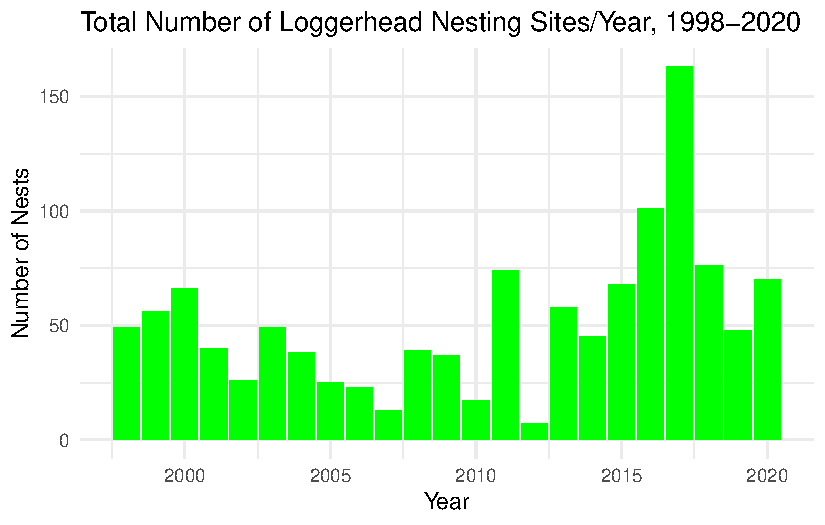
\includegraphics{RAWH_CAPSTONE_041926_files/figure-pdf/fig-total-nesting-year-1.pdf}

}

\caption{\label{fig-total-nesting-year}Total Number of Loggerheads
Nesting Sites/Year, 1998-2020}

\end{figure}%

\begin{figure}

\centering{

\begin{table}
\caption*{
{\fontsize{20}{25}\selectfont  Beach Area Nest Totals\fontsize{12}{15}\selectfont }
} 
\fontsize{12.0pt}{14.0pt}\selectfont
\begin{tabular*}{\linewidth}{@{\extracolsep{\fill}}lr}
\toprule
Location & Nest Total \\ 
\midrule\addlinespace[2.5pt]
Perdido Key & 366 \\ 
Santa Rosa Beach & 301 \\ 
Pensacola Beach & 278 \\ 
Fort Pickens & 243 \\ 
\bottomrule
\end{tabular*}
\end{table}

}

\caption{\label{fig-beach-table}Area Totals of Loggerhead Turtle Nesting
Sites: 1998-2020}

\end{figure}%

\begin{figure}

\centering{

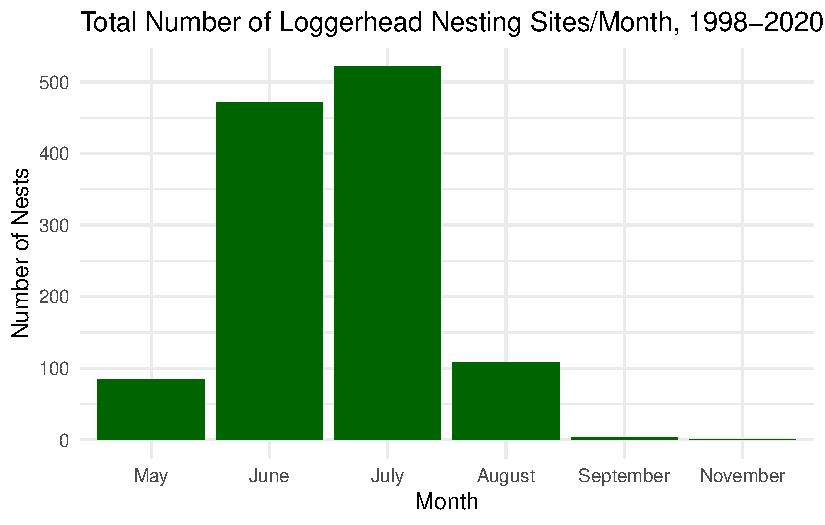
\includegraphics{RAWH_CAPSTONE_041926_files/figure-pdf/fig-top-month-1.pdf}

}

\caption{\label{fig-top-month}Total Number of Loggerhead Nesting
Sites/Month, 1998-2020}

\end{figure}%

\begin{figure}

\centering{

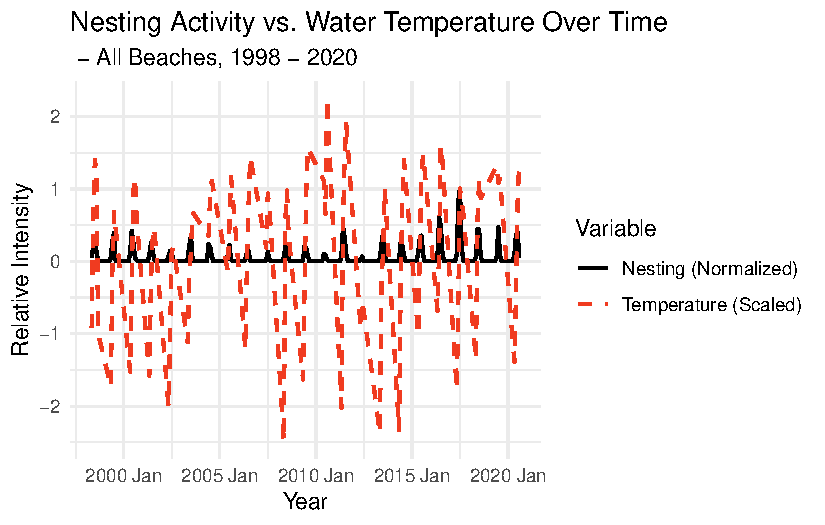
\includegraphics{RAWH_CAPSTONE_041926_files/figure-pdf/fig-relative-nest-temp-1.pdf}

}

\caption{\label{fig-relative-nest-temp}Relative Relationship of Nesting
Activity vs Average Temperatures, 1988-2020}

\end{figure}%

\begin{table}

\caption{\label{tbl-CCseason-table}Seasonal Start/End Dates and Total
Number of Nesting Sites for Each Season: 1988-2020}

\centering{

\caption*{
{\fontsize{20}{25}\selectfont  Annual Loggerhead Nesting Season Dates\fontsize{12}{15}\selectfont } \\ 
{\fontsize{14}{17}\selectfont  - 1998-2020, Gulf Coast Study Area\fontsize{12}{15}\selectfont }
} 
\fontsize{12.0pt}{14.0pt}\selectfont
\begin{tabular*}{\linewidth}{@{\extracolsep{\fill}}cccc}
\toprule
Year & Start Date & End Date & Total Sites \\ 
\midrule\addlinespace[2.5pt]
1998 & 10369 & 10475 & 49 \\ 
1999 & 10735 & 10792 & 56 \\ 
2000 & 11086 & 11222 & 65 \\ 
2001 & 11469 & 11546 & 40 \\ 
2002 & 11810 & 11911 & 26 \\ 
2003 & 12193 & 12268 & 49 \\ 
2004 & 12577 & 12648 & 38 \\ 
2005 & 12938 & 13006 & 25 \\ 
2006 & 13293 & 13367 & 23 \\ 
2007 & 13691 & 13731 & 13 \\ 
2008 & 14020 & 14111 & 39 \\ 
2009 & 14382 & 14477 & 37 \\ 
2010 & 14767 & 14826 & 17 \\ 
2011 & 15113 & 15207 & 74 \\ 
2012 & 15483 & 15498 & 7 \\ 
2013 & 15836 & 15931 & 58 \\ 
2014 & 16210 & 16312 & 45 \\ 
2015 & 16568 & 16678 & 68 \\ 
2016 & 16939 & 17044 & 101 \\ 
2017 & 17302 & 17414 & 163 \\ 
2018 & 17670 & 17754 & 76 \\ 
2019 & 18075 & 18138 & 48 \\ 
2020 & 18404 & 18491 & 70 \\ 
\bottomrule
\end{tabular*}

}

\end{table}%

\begin{figure}

\centering{

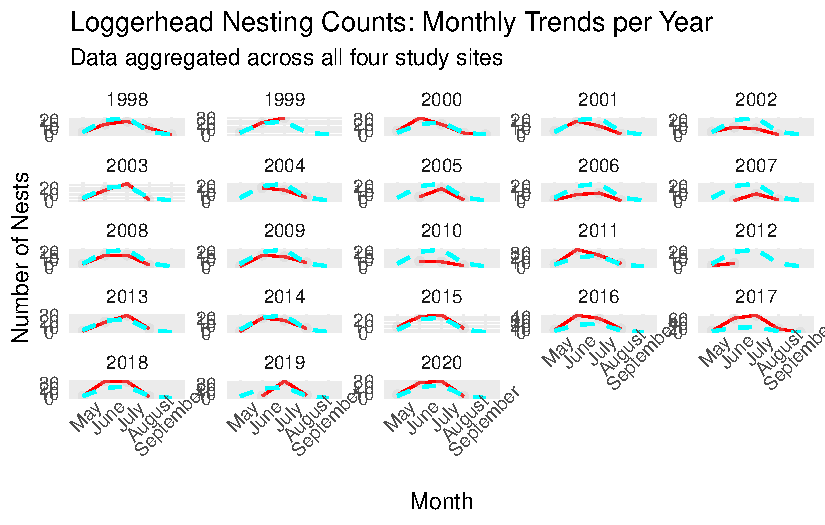
\includegraphics{RAWH_CAPSTONE_041926_files/figure-pdf/fig-ind-plots-1.pdf}

}

\caption{\label{fig-ind-plots}Individual Plots for each Season:
1988-2020}

\end{figure}%

\phantomsection\label{refs}
\begin{CSLReferences}{1}{0}
\bibitem[\citeproctext]{ref-BoxJenkins1970}
Box, \& Jenkins, G. E. P. 1970. \emph{Time Series Analysis: Forecasting
and Control}. San Francisco, CA: Holden-Day.

\bibitem[\citeproctext]{ref-fpp3}
Hyndman, Rob J., and George Athanasopoulos. 2026. \emph{Forecasting:
Principles and Practice}.
\url{https://otexts.com/fpp3/https://otexts.com/fpp3/}.

\bibitem[\citeproctext]{ref-MathWorks}
MathWorks. 2026. {``Time Series Analysis.''} 2026.
\url{https://www.mathworks.com/discovery/time-series-analysis.html}.

\bibitem[\citeproctext]{ref-Mazaris2004}
Mazaris, Matsinos, Kornaraki. 2004. {``Modeling the Effect of Sea
Surface Temperature on Sea Turtle Nesting Activities by Investigating
Seasonal Trends.''} \emph{Natural Recourse Modeling}.

\end{CSLReferences}




\end{document}
